\documentclass[t]{beamer}

\usetheme{Air}
\usepackage{graphics}
\usepackage{graphicx}
\graphicspath{{C:/Users/Brayden/Projects/PEPS-Data/}{.}}
%\usepackage{caption}
\usepackage{amsthm}
%\usepackage{thumbpdf}
\usepackage{wasysym}
\usepackage{ucs}
\usepackage[utf8]{inputenc}
\usepackage{pgf}
\usepackage{verbatim}
\usepackage{tikz}
\usepackage{pgfmath}
\usetikzlibrary{calc}
\usetikzlibrary{backgrounds}
\usetikzlibrary{arrows}
\usetikzlibrary{shapes.arrows}
\usetikzlibrary{shapes.geometric}
\usetikzlibrary{decorations.markings}
\usetikzlibrary{positioning}
\usetikzlibrary{fit,chains}
\usepackage{natbib}
\usepackage{wasysym}
\usepackage{soul} 
\bibliographystyle{apalike}  

%\usepackage{pstricks}
%\newpsobject{psid}{psline}{linestyle=dotted,dotsep=1pt}
%\newpsobject{pspsi}{psline}{doubleline=true}
%\newpsobject{pssigma}{psline}{linewidth=1.5pt}

%\usepackage{pgfpages}
%\setbeamertemplate{note page}[plain]
%\setbeameroption{show notes on second screen=right}
%http://tex.stackexchange.com/questions/21777/is-there-a-nice-solution-to-get-a-presenter-mode-for-latex-presentations

\newcommand{\beq}{\begin{equation}}
\newcommand{\eeq}{\end{equation}}
\newcommand{\beqa}{\begin{eqnarray}}
\newcommand{\eeqa}{\end{eqnarray}}
\newcommand{\bi}{\begin{itemize}}
\newcommand{\ei}{\end{itemize}}
\newcommand{\ket} [1] {\vert #1 \rangle}
\newcommand{\bra} [1] {\langle #1 \vert}
\newcommand{\braket}[2]{\langle #1 | #2 \rangle}
\newcommand{\ev}[1]{\langle #1 \rangle}
\newcommand{\vbra}[1]{\left ( #1 \right |}
\newcommand{\vket}[1]{\left |#1 \right )}
\newcommand{\vbraket}[2]{\left ( #1 \middle |#2 \right )} 
\newcommand{\braopket}[3]{\left \langle #1 \middle |#2 \middle | #3 \right \rangle} 
\newcommand{\vbraopket}[3]{\left ( #1 \middle |#2 \middle | #3 \right )} 

%\newcommand<>{\highlighton}[1]{%
%  \alt#2{\structure{#1}}{{#1}}
%}

\newcommand{\icon}[1]{\pgfimage[height=1em]{#1}}

\usepackage{empheq}

\newlength\mytemplen
\newsavebox\mytempbox

\makeatletter
\newcommand\mybluebox{%
    \@ifnextchar[%]
       {\@mybluebox}%
       {\@mybluebox[0pt]}}

\def\@mybluebox[#1]{%
    \@ifnextchar[%]
       {\@@mybluebox[#1]}%
       {\@@mybluebox[#1][0pt]}}

\def\@@mybluebox[#1][#2]#3{
    \sbox\mytempbox{#3}%
    \mytemplen\ht\mytempbox
    \advance\mytemplen #1\relax
    \ht\mytempbox\mytemplen
    \mytemplen\dp\mytempbox
    \advance\mytemplen #2\relax
    \dp\mytempbox\mytemplen
    \fcolorbox{airlightblue}{white}{\hspace{1em}\usebox{\mytempbox}\hspace{1em}}}

\makeatother

\tikzset{peps/.style={circle=2pt,draw=black!100,fill=green!50,inner sep=3pt}}
\tikzset{bpeps/.style={circle=2pt,draw=black!100,thick,fill=green!50,inner sep=3pt}}
\tikzset{gamma/.style={circle=2pt,draw=black!100,fill=blue!20,inner sep=3pt}}
\tikzset{lambda/.style={rectangle,rotate=45,draw=black!100,fill=orange!50,inner sep=4pt}}
\tikzset{operator/.style={circle=2pt,draw=black!100,fill=orange!80,inner sep=3pt}}
\tikzset{cdot/.style={circle=2pt,draw=black!100,fill=white,inner sep=1pt}}
\tikzset{bg/.style={rounded corners,thin,fill=blue!10}}
\tikzset{inv/.style={opacity=0}}
\tikzset{spin/.style={circle=2pt,draw=black!100,fill=orange!80,inner sep=3pt}}
\tikzset{unitbox/.style={fill=black!3,rounded corners}}
\tikzset{corner/.style={rectangle=10pt,fill=blue!50,draw=black}}
\tikzset{side/.style={rectangle=6pt,fill=blue!20,draw=black}}
\tikzset{cside/.style={circle=6pt,fill=blue!20,draw=black}}
\tikzset{swapg/.style={circle=1pt,draw=black,fill=black!80,inner sep=1pt}}

\tikzset{base/.style={circle=2pt,fill=orange!80,draw=black}}
\tikzset{det/.style={circle=2pt,fill=blue!20,draw=black,inner sep=4pt}}
\tikzset{iso/.style={circle=2pt,fill=red!20,draw=black,inner sep=4pt}}
\tikzset{top/.style={circle=2pt,fill=black!20,draw=black,inner sep=4pt}}
\tikzset{siso/.style={circle=1pt,fill=red!20,draw=black,inner sep=1pt}}

%Brayden's
\tikzset{GHZ/.style={circle=2pt,fill=black!80,draw=black,inner sep=2pt}}
\tikzset{X/.style={circle=2pt,fill=black!80,text=white,font=\footnotesize, draw=black,inner sep=1pt}}
\tikzset{W/.style={circle=2pt,fill=black!20,draw=black,double,inner sep=2pt}}
\tikzset{eli/.style={ellipse, rotate=0, draw=black, fill=gray!20}}

%http://tex.stackexchange.com/questions/199683/how-to-plot-quantum-logical-gates-with-tikz
\tikzset{
cross/.style={path picture={ 
            \draw[thick,black](path picture bounding box.north) -- (path picture bounding                  box.south) (path picture bounding box.west) -- (path picture bounding                      box.east);
            }},
crossx/.style={path picture={ 
            \draw[thick,black,inner sep=0pt]
                (path picture bounding box.south east) -- (path picture bounding box.north west) (path picture bounding box.south west) -- (path picture bounding box.north east);
            }},
circlewc/.style={circle=2pt,draw, crossx}
}
%\newtheorem{LSM}{{\em Theorem: Lieb, Schultz, Mattis (1961)}}
%\newtheorem{Oshikawa}{{\em Extension: Oshikawa (1999)}}

\pdfinfo
{
  /Title       (Entanglement in Featureless Mott Insulators)
  /Creator     (TeX)
  /Author      (Brayden Ware)
}


\title{Entanglement in Featureless Mott Insulators}
%\subtitle{}
\author{Brayden Ware}
\date{September 26th 2014}

%\includeonly{slides/LSM1}
\begin{document}

\frame{\titlepage}


%%%%%%%%%%%%%%%%%%%%%%%%%%%%%%%%%%%%%%%%%
%%%%%%%%%% Pre-outline section %%%%%%%%%%
%%%%%%%%%%%%%%%%%%%%%%%%%%%%%%%%%%%%%%%%%
% \section*{}

% \begin{frame}{Frame Title}
\vskip-1.5cm

\end{frame}

%%%%%%%%%%%%%%%%%%%%%%%%%%%%%%%%%%%%%%%%%
%%%%%%%%%% Outline code %%%%%%%%%%%%%%%%%
%%%%%%%%%%%%%%%%%%%%%%%%%%%%%%%%%%%%%%%%%
\section*{}

\begin{frame}
  \frametitle{Outline}
  \vskip-1.5cm
  \tableofcontents
\end{frame}

\AtBeginSection[]
{
\frame{
  \vspace{2cm}
  {\huge \insertsection}
  }
}
%\AtBeginSection[]
%{
%  \frame<handout:0>
%  {
%    \frametitle{Outline}
%    \vskip-1.5cm
%    \tableofcontents[currentsection]
%  }
%}

%\AtBeginSubsection[]
%{
%  \frame<handout:0>
%  {
%    \frametitle{Outline}
%    \tableofcontents[sectionstyle=show/hide,subsectionstyle=show/shaded/hide]
%  }
%}
%%%%%%%%%%%%%%%%%%%%%%%%%%%%%%%%%%%%%%%%%
%%%%%%%%%% Content starts here %%%%%%%%%%
%%%%%%%%%%%%%%%%%%%%%%%%%%%%%%%%%%%%%%%%%

\section{Motivation}
\begin{frame}{Featureless Insulators}
\vskip-1.5cm
\begin{columns}[T]
    \begin{column}[T]{.6\textwidth}
        \begin{block}{Definition of `Featureless Insulator'}
            \vskip-1em
            \begin{itemize}
                % 0 T G.S. of quantum Hamiltonians
            \item Gapped 
                %Energy gap to excitations
            \item Symmetric 
                %G.S. Wavefunc preserves all symmetries of the Hamiltonian, no local order parameter - no spontaneous symmetry breaking
            \item No topological order %exotic statistics
                %insulator ->assume that we have a U(1) symmetry by which to define charge
            \item Integer charge per unit cell
                %unit cell -> also assuming discrete translational symmetry
            \item Unique ground state with P.B.C.
                %This can be made into the defining property, all of these others follow from this.
                % Response to change in B.C. can be, with some work, a way to distinguish gapped phases of matter
            \end{itemize}
        \end{block}
    \vskip-0.5cm    
    Examples:
    \end{column}
    \begin{column}[T]{.4\textwidth}
    \begin{figure}[h]
            \centering
            \scalebox{0.7}{
            %
% x=3*(minimum size)/2
% y=\sqrt{3/4}*(minimum size)/2
%

%http://tex.stackexchange.com/questions/6019/drawing-hexagons
\begin{tikzpicture}[x=7.5mm,y=4.33mm]
  % some styles
  \tikzset{
    box/.style={
      regular polygon,
      regular polygon sides=6,
      minimum size=10mm,
      inner sep=0mm,
      outer sep=0mm,
      rotate=0,
    draw
    }
  }
 \tikzset{boson/.style={circle=1pt,draw=black!100,fill=orange!100,inner sep=2pt}}

\foreach \i in {0,...,2} 
    \foreach \j in {0,...,3} {
            \node[box] at (2*\i,2*\j) {};
        }
\foreach \i in {0,...,1} 
    \foreach \j in {0,...,2} {
   	   \node[box] at (2*\i+1,2*\j+1) {};   
        }
\foreach \i in {0,...,2} 
    \foreach \j in {0,...,3} {
            \node[boson] at (2*\i-0.6,2*\j) {};
            \node[boson] at (2*\i+0.6,2*\j) {};
            \node[boson] at (2*\i-0.4,2*\j-1) {};
            \node[boson] at (2*\i-0.4,2*\j+1) {};
             \node[boson] at (2*\i+0.4,2*\j+1) {};
              \node[boson] at (2*\i+0.4,2*\j-1) {};
        }
%\foreach \i in {0,...,1} 
  %  \foreach \j in {0,...,2} {
%	\node[boson] at (2*\i+1-0.6,2*\j+1) {}; 
%	\node[boson] at (2*\i+1+0.6,2*\j+1) {};   
   %   }
      
\end{tikzpicture}

            }
            %Atomic insulator
            \caption{\begin{tabular}[t]{l}
                     Bosonic Mott insulator \\
                     with integer filling \end{tabular}}
    \end{figure}
    \end{column}
\end{columns}

\begin{columns}[T]
    \begin{column}[T]{.4\textwidth}
        \vskip-0.5cm
        \begin{figure}[h]
            \centering
            \scalebox{0.6}{
             \begin{tikzpicture}[domain=0:6.28]
      \draw[very thick] (0, -2.5) -- (0,1) node[left, midway] {\LARGE $E$} ;
      \draw[very thick] (0, 1)-- (6.28,1) -- (6.28, -2.5) -- (0, -2.5);
      \draw[color=black, very thick] plot (\x,{-1+cos(\x r)}) node[right] {};
      \draw[color=orange, fill] plot (\x,{-0.95+cos(\x r)}) {};
  \end{tikzpicture}
  
            }
        \caption{Band Insulator}
        \end{figure}
    \end{column}
    \begin{column}[T]{.6\textwidth}
        \begin{figure}[h]
            \scalebox{1.4}{
            \tikzset{eli/.style={ellipse, rotate=0, draw=black, fill=gray!20}}
\tikzset{button/.style={
% First preaction: Fuzzy shadow
preaction={fill=black,path fading=circle with fuzzy edge 20 percent,
opacity=.5,transform canvas={xshift=1mm,yshift=-1mm}},
% Second preaction: Background pattern
preaction={pattern=#1,
path fading=circle with fuzzy edge 15 percent},
% Third preaction: Make background shiny
preaction={top color=white,
bottom color=black!50,
shading angle=45,
path fading=circle with fuzzy edge 15 percent,
opacity=0.2},
% Fourth preaction: Make edge especially shiny
preaction={path fading=fuzzy ring 15 percent,
top color=black!5,
bottom color=black!80,
shading angle=45},
inner sep=2ex
},
button/.default=horizontal lines light blue,
circle}
\usetikzlibrary{backgrounds}
\pgfdeclarelayer{background}
\pgfsetlayers{background,main}
\begin{tikzpicture}
\begin{scope}[on background layer]
\node[eli] at (0,0) {$\,\,\,$};
\node[eli] at (0.7,0) {$\,\,\,$};
\node[eli] at (1.4,0) {$\,\, \,$};
\node[eli] at (2.1,0) {$\,\, \,$};
\end{scope}

\node[inv] (s0) at (-0.1, -0.1){};
\node[inv] (t0) at (-0.1,  0.1){};
\path[->, thick, orange] (s0.center) edge (t0.center);

\node[inv] (s1) at (0.1, -0.1){};
\node[inv] (t1) at (0.1,  0.1){};
\path[->, thick, orange] (s1.center) edge (t1.center);

\node[inv] (s2) at (0.6, -0.1){};
\node[inv] (t2) at (0.6,  0.1){};
\path[<-, thick, orange] (s2.center) edge (t2.center);

\node[inv] (s3) at (0.8, -0.1){};
\node[inv] (t3) at (0.8,  0.1){};
\path[->, thick, orange] (s3.center) edge (t3.center);

\node[inv] (s4) at (1.3, -0.1){};
\node[inv] (t4) at (1.3,  0.1){};
\path[<-, thick, orange] (s4.center) edge (t4.center);

\node[inv] (s5) at (1.5, -0.1){};
\node[inv] (t5) at (1.5,  0.1){};
\path[->, thick, orange] (s5.center) edge (t5.center);

 \node[inv] (s6) at (2.0, -0.1){};
 \node[inv] (t6) at (2.0,  0.1){};
\path[<-, thick, orange] (s6.center) edge (t6.center);

\node[inv] (s7) at (2.2, -0.1){};
\node[inv] (t7) at (2.2,  0.1){};
\path[<-, thick, orange] (s7.center) edge (t7.center);

\foreach \i in {0, 1, 2, 3}{
\node[inv] (u\i) at (0.7*\i-0.1, 0){};
\node[inv] (v\i) at (0.7*\i+0.1, 0){};
}
\node[inv] (u4) at (0.7*4-0.2, 0){};
\node[inv] (vm1) at (-0.5, 0){};

\draw[color=black] (vm1.center)  -- (u0.center);
\draw[ color=black] (v0.center)  -- (u1.center);
\draw[ color=black] (v1.center)  -- (u2.center);
\draw[ color=black] (v2.center)  -- (u3.center);
\draw[color=black] (v3.center)  -- (u4.center);

\node[] at (-0.7, 0){...};
\node[] at (2.8, 0){...};

\end{tikzpicture}
            }
            \caption{Heisenberg AF Spin-1 chain}
        \end{figure}
    \end{column}
\end{columns}
\end{frame}
%\subsection{Band Insulators}
\newcommand{\kk}{\mathbf{k}}
\begin{frame}{Free Fermion Band Insulators}
\vskip-1.5cm
\begin{columns}[T]
\begin{column}[T]{0.65\textwidth}
\bi 
\item Crystalline, 0T insulators \\(including semiconductors)
%A good source of examples - column IV of periodic table, such as C, or in combination with column VI 
%(Columns I-III prefer to donate their valence electrons and form ionic bonds or metals)
%Microscopics are described well by
\item Tight-binding Hamiltonian 
$$
\mathcal{H}_{FF} =  \sum\limits_{<ij>}\sum\limits_{\alpha, \beta}-t_{\alpha, \beta} c^{\alpha \dagger}_{i} c_{j}^{\beta} - \mu \sum\limits_{i, \alpha} N_{i}^{\alpha} 
$$
%Diagonalize in momentum space to produce band picture, completely fill some lowest number of bands
\item Bloch wavefunctions
$
\ket{u^{\alpha}_{\kk}}
$
%Low energy physics can be described by the Dirac Hamiltonian, with an effective mass for electron-like excitations, which looks in 2d like
\item Massive Dirac Hamiltonian 
$$
\mathcal{H}_{D}(\kk) = \kk_x \sigma_x + \kk_y \sigma_y + m_*\sigma_z
$$
%Describing a single conduction and valence band with a gap to pair production of quasi-electron+quasi-hole
\item Atomic-insulating like Wannier basis
%From Fourier transforming the Block wavefunctions
\item Density plateau
\ei 
\end{column}

\begin{column}[T]{0.35\textwidth}
\only<1->{
    \begin{figure}
        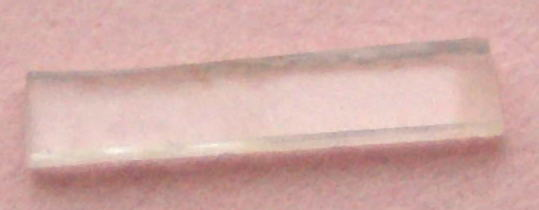
\includegraphics[width=\linewidth]{diagrams/GaNcrystal.jpg}
        \caption{Semiconductor GaN}
    \end{figure}
}
\vskip-0.5cm    
\only<1>{
    \begin{figure}
        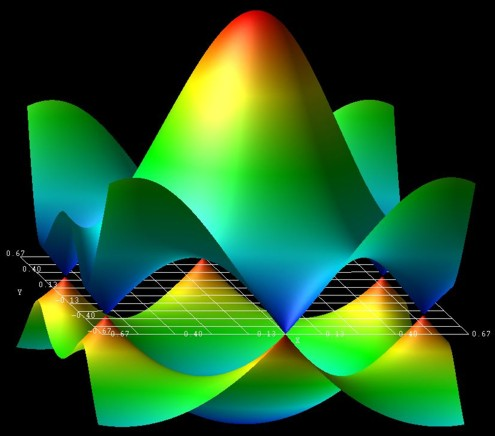
\includegraphics[width=\linewidth]{diagrams/grapheneband2.jpg}
        \caption{Band Theory}
    \end{figure}
}
% \only<3>{
    % \begin{figure}
        % 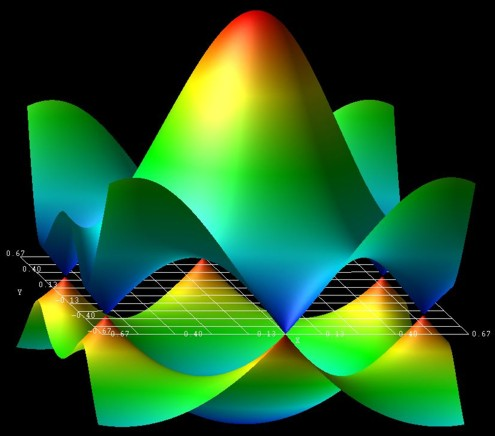
\includegraphics[width=\linewidth]{diagrams/grapheneband2.jpg}
        % \caption{Dirac Band Theory}
    % \end{figure}
% } 
\only<2>{
    \begin{figure}
        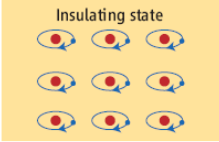
\includegraphics[width=\linewidth]{diagrams/bernevig1.png}
        \caption{Atomic Insulator}
    \end{figure}
}
\only<3>{
    \begin{figure}
        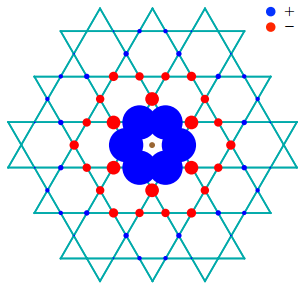
\includegraphics[width=\linewidth]{diagrams/kagomewannier.png}
        \caption{Wannier Function}
    \end{figure}
}
\end{column}
\end{columns}
\end{frame}
\begin{frame}{Free Fermion Band Insulators}
\vskip-1.5cm
\begin{columns}[T]
\begin{column}[T]{0.65\textwidth}
\end{column}
\end{columns}
\end{frame}
\begin{frame}{$\mathcal{T}$-Symmetric Honeycomb Band Insulators}
\vskip-1.5cm
\begin{columns}
\begin{column}[T]{0.65\textwidth}
%Famously
From considerations of graphene, a tight-binding honeycomb lattice model of fermions:

\bi
\item A spinless fermion has protected Dirac points
\bi
\item with $\mathcal{I}$ and $\mathcal{T}$ symmetry
\item NO featureless insulators at filling 1 on the honeycomb lattice with $\mathcal{T}$
%One way to say it: T guarantees m = m' where m and m' are the effective masses at the special momenta labeled K and K'
% On the otherhand, I guarantees m=-m' and with T broken gives a chern number \pm1. 
\ei 
\item<2-> Breaking  $\mathcal{T}$ leads to non-zero Chern number - $\mathbb{Z}$ invariant, QAHE 
%Haldane proposed using complex hopping amplitudes to do this in 1988 instead of a static magnetic field, QAHE -IQHE without net magnetic flux

%This situation can be exploited to make something new, by taking two copies.
\item<3-> Spinful fermions with spin-orbit couplings have two bands, with Chern numbers $\pm 1$.
%Net chern number and qhconductance is zero but there is quantum spin hall current
%Charlie Kane 2004
%2d topological insulator, edge is a kramers doublet in general
\item<3-> $\mathbb{Z}_2$ topological invariant 
\vskip-0.3cm
\ei
\end{column}
\begin{column}[T]{0.35\textwidth}
\only<1>{
    \begin{figure}
        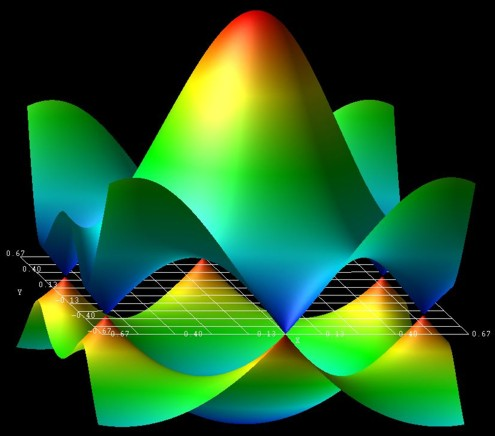
\includegraphics[width=\linewidth]{diagrams/grapheneband2.jpg}
        \caption{Dirac Points}
    \end{figure}
    \vskip-2cm
        \begin{figure}
        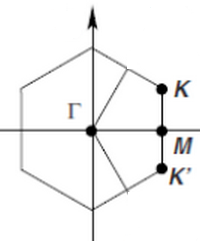
\includegraphics[width=\linewidth]{diagrams/kpoint.png}
        \caption{Brillouin Zone}
    \end{figure}
}
\only<2->{
\begin{figure}
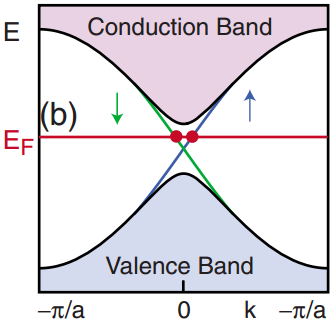
\includegraphics[width=\linewidth]{diagrams/helical_edge.png}
\caption{Helical Edge \footnotemark}
\end{figure}
\vskip-0.5cm
\bi 
\item $\mathcal{T}$-symmetric quantum spin-hall insulator.
%spin-hall conductance is non-zero
%edges can be gapped out by breaking T
\ei }
\end{column}
\end{columns}
\footnotetext[2]{
\citep{Hasan2010-fq}} 
\end{frame}
\begin{frame}{Free Fermion Edge Classification}
\vskip-1.5cm
\only<1>{
By partitioning the wavefunction, we can glimpse the edge
\begin{columns}[T]
\begin{column}{0.5\textwidth}
\begin{figure}
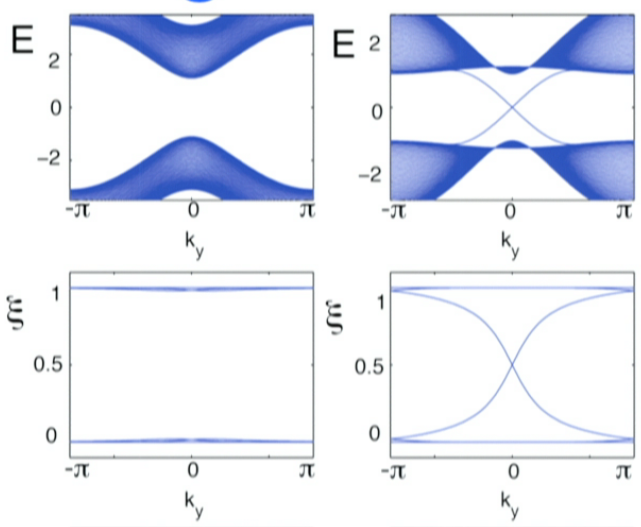
\includegraphics[width=\linewidth]{diagrams/QSH.png}
\caption{Top: Physical spectrum with boundary.
Bottom: 'Single particle entanglement spectrum'}
\end{figure}
\end{column}
\begin{column}{0.5\textwidth}
\bi
\item $G_{ij} = \ev{c^{\dagger}_i c_j}$ 
%\item Determines free fermion state
%\item Eigenvalues are 1, 0
\item $G^L_{ij}$ is G restricted to left half of cylinder
\item Spectrum of $G^L$ shown.
\item 'Gapless entanglement mode' protected by $\mathcal{T}$

\item Bulk wavefunction E.S. shown to capture edge physics
\item Bulk wavefunction shown to be distinct from atomic insulator
\ei 

\end{column}
\end{columns}
}
\only<2>{
    Results for free fermions without lattice symmetries:
    \begin{figure}
    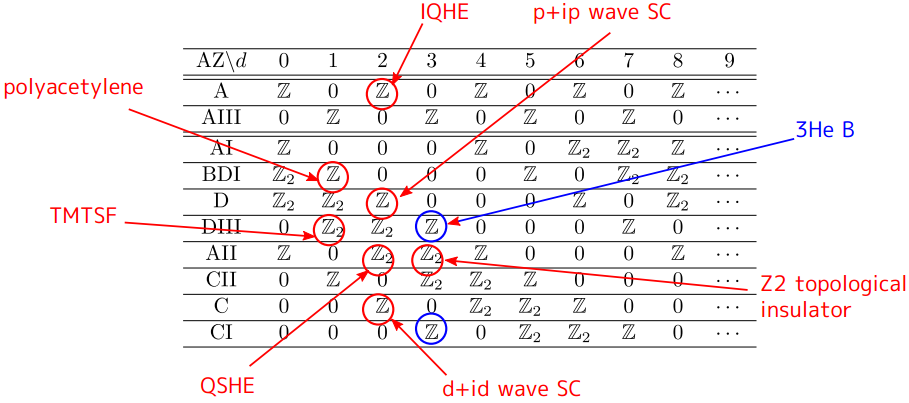
\includegraphics[width=\linewidth]{diagrams/AZ.png}
    \caption{Free-fermion classification (ten-fold way) for $       \mathcal{T}, \mathcal{C}$} 
    \end{figure}
    \footnotetext[5]{
    \citep{Ryu2009-qc}} 
%These invariants aren't always very physical, and while they distinguish free fermion Hamiltonians, they aren't guaranteed to stick around when you add interactions.

% Most of the invariants are only well defined in the presence of some additional symmetry

% There is an big table of free-fermion classification called the 10 fold way for time-reversal and charge conjugation symmetry, and a bigger table when you include lattice symmetries (Topological Crystalline Insulators)
}


\end{frame}
\begin{frame}{Motivating Questions}
\vskip-1.5cm
%We want to classify and understand all featureless insulators, 
%but thats a big undertaking so lets break that question down into some smaller questions.


\begin{block}{Existence}
Fix a lattice $\Lambda$, symmetry group $G$, and integer filling number $m$

Do there exist any featureless insulators at all?
\bi 
\item Find \textbf{obstruction} to existence
\item or \textbf{construct} a reference featureless insulator
\ei 
%The Lieb-Schultz-Mattis theorem gives one such constraint - m must be an integer. Is that the only constraint? Can you prove it by constructing featureless insulators for every m? You might try to construct one and realize that there are additional obstructions that you haven't thought of yet, which would allow you to extend the LSM theorem.
\end{block}

\begin{block}{Characterization}
Given a quantum wavefunction, is it a featureless insulator? Is it distinguishable from atomic insulator in the presence of a symmetry group $G$? What is $G$?

\bi
\item Show non-trivial protected physical or entanglement edge modes 
\item Find a topological invariant that distinguishes it
\ei 
\end{block}
\end{frame}
%\subsection{Bosonic Mott Insulators}
\begin{frame}{Bosonic Mott Insulators}
\vskip-1.5cm

\only<1>{
        \begin{figure}
        \centering
        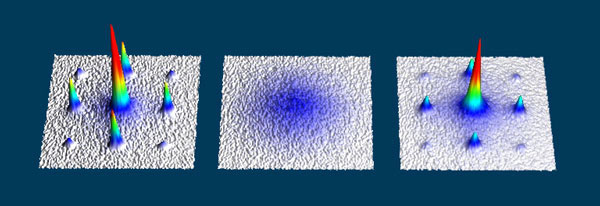
\includegraphics[width=\linewidth]{diagrams/SuperfluidStates.jpg}
        \caption{Mott insulator with cold atoms in optical lattice\footnotemark}
        \end{figure}
        }
\begin{block}{Bose-Hubbard model}
\vskip-0.3cm
$$
H_{BH} = -J \sum\limits_{<ij>} b^{\dagger}_i b_j - \mu \sum\limits_i N_i + \frac12 V \sum\limits_i N_i (N_i-1)
$$
\end{block}
\only<2->{
\begin{columns}[T]
    \begin{column}[T]{.4\textwidth}
        \vskip-1.2cm

        \only<2>{
        \begin{figure}
        \centering
        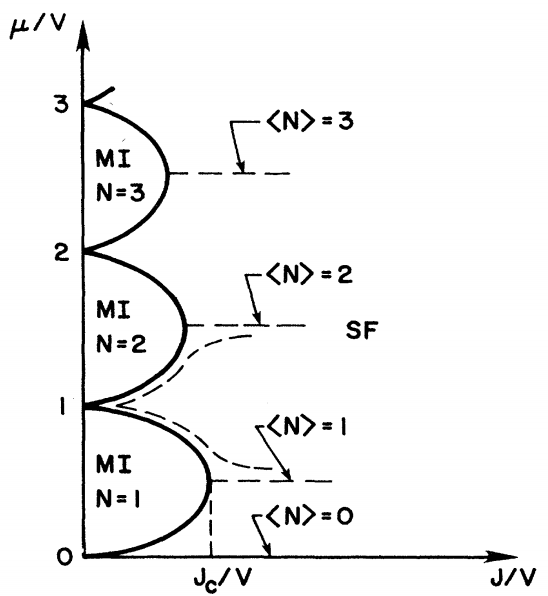
\includegraphics[width=\linewidth]{diagrams/bosehubbard2.png}
        \end{figure}
        }
    \end{column}
    \begin{column}[T]{.6\textwidth}
    \vskip-0.7cm
    \bi
    \item Form an atomic insulator with N bosons to minimize $-\mu N + VN(N-1)/2$
    %Particles and holes have a cost based on this function
    %particle cost goes to zero at transition between fillings
    \item Gap to particle/hole excitations
    %Kinetic energy causes some local density fluctuations, but not much else
    \item Bosons free to hop will instantly condense into superfluid with any $J$
    %Must have interactions, and in cold atoms
    %Deep optical lattice wells to keep $J$ small enough
    \item Number conserving - so no superfluid phase coherence
    %\item Unlike free-fermions, not obvious how to construct fractional site filling insulators
    %\item Tensor network states give us access to needed construction and to interacting invariants.
    %\note{LSM inspired invariants}
    \ei
    \end{column}
\end{columns}
}
\only<1>{
\footnotetext[3]{\citep{Greiner2002-ay}}
}
\only<2>{
\footnotetext[4]{\citep{Fisher1989-ou}}
}
\end{frame}

%\subsection{Honeycomb Bosonic Mott Insulators?}
\begin{frame}{Honeycomb Bosonic Mott Insulators}
\vskip-1.5cm
Does there exist a featureless bosonic insulator with charge 1 per unit cell on the honeycomb lattice?
%Is it possible to extend the Lieb Schultz Mattis theorem in this case
\only<1>{
\begin{columns}[T]
	\begin{column}[T]{.5\textwidth}
		\begin{figure}
			\scalebox{1}{
			%
% x=3*(minimum size)/2
% y=\sqrt{3/4}*(minimum size)/2
%

%http://tex.stackexchange.com/questions/6019/drawing-hexagons
\begin{tikzpicture}[x=7.5mm,y=4.33mm]
  % some styles
  \tikzset{
    box/.style={
      regular polygon,
      regular polygon sides=6,
      minimum size=10mm,
      inner sep=0mm,
      outer sep=0mm,
      rotate=0,
    draw
    }
  }
 \tikzset{boson/.style={circle=1pt,draw=black!100,fill=orange!100,inner sep=2pt}}

\foreach \i in {0,...,2} 
    \foreach \j in {0,...,3} {
            \node[box] at (2*\i,2*\j) {};
        }
\foreach \i in {0,...,1} 
    \foreach \j in {0,...,2} {
   	   \node[box] at (2*\i+1,2*\j+1) {};   
        }
\foreach \i in {0,...,2} 
    \foreach \j in {0,...,3} {
            \node[boson] at (2*\i-0.6,2*\j) {};
           % \node[boson] at (2*\i+0.6,2*\j) {};
           % \node[boson] at (2*\i-0.4,2*\j-1) {};
           % \node[boson] at (2*\i-0.4,2*\j+1) {};
             \node[boson] at (2*\i+0.4,2*\j+1) {};
              \node[boson] at (2*\i+0.4,2*\j-1) {};
        }
%\foreach \i in {0,...,1} 
  %  \foreach \j in {0,...,2} {
%	\node[boson] at (2*\i+1-0.6,2*\j+1) {}; 
%	\node[boson] at (2*\i+1+0.6,2*\j+1) {};   
   %   }
      
\end{tikzpicture}

			}\caption{Breaks rotational symmetry}
		\end{figure}
	\end{column}
	\begin{column}[T]{.5\textwidth}
		\begin{figure}
			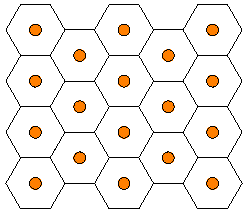
\includegraphics[width=.8\textwidth]{diagrams/hex_center_honeycomb.pdf}
			\caption{Leaves honeycomb lattice}
		\end{figure}
	\end{column}
\end{columns}
}
\only<2>{
\begin{figure}
\scalebox{1}{
% y=\sqrt{3/4}*(minimum size)/2
%

%http://tex.stackexchange.com/questions/6019/drawing-hexagons
\begin{tikzpicture}[x=7.5mm,y=4.33mm]
  % some styles
  \tikzset{
    box/.style={
      regular polygon,
      regular polygon sides=6,
      minimum size=10mm,
      inner sep=0mm,
      outer sep=0mm,
      rotate=0,
      dotted,
      thick,
      black,
      draw
    }
  }
 \tikzset{boson/.style={circle=1pt,draw=black!100,fill=orange!100,inner sep=2pt}}
  \tikzset{dimer/.style={ellipse=1pt,draw=black!100,fill=orange!90,inner sep=2pt}}
    \tikzset{thindimer/.style={ellipse=1pt,draw=black!100,fill=orange!90,inner sep=1pt}}

\foreach \i in {0,...,2} 
    \foreach \j in {0,...,3} {
            \node[box] at (2*\i,2*\j) {};
        }
\foreach \i in {0,...,1} 
    \foreach \j in {0,...,2} {
   	   \node[box] at (2*\i+1,2*\j+1) {};   
        }

 \foreach \i in {-1,...,2} 
     \foreach \j in {-1,...,2} 
     {
     \pgfmathtruncatemacro{\xa}{2*\i + 1*\j}
     \pgfmathtruncatemacro{\ya}{3*\j}
      \pgfmathtruncatemacro{\xb}{2*\i + 1*\j+1}
     \pgfmathtruncatemacro{\yb}{3*\j+1}
      \pgfmathtruncatemacro{\xc}{2*\i + 1*\j}
     \pgfmathtruncatemacro{\yc}{3*\j+2}
    
    \ifnum -1<\xa \ifnum \xa<5
     \ifnum\ya<7\ifnum-1<\ya 
	% \node[thindimer, rotate=120] at (\x-1/2,\y-1/2) {$\,\,\,\,$};     
     %\node[thindimer, rotate=120] at (\x+1/2,\y+1/2) {$\,\,\,\,$};
     %\node[thindimer, rotate=60] at (\x-1/2,\y+1/2) {$\,\,\,\,$};
       %\node[thindimer, rotate=60] at (\x+1/2,\y-1/2) {$\,\,\,\,$};
     \node[thindimer, rotate=0] at (\xa,\ya-1) {$\,\,\,\,$};
      \node[thindimer, rotate=0] at (\xa,\ya+1) {$\,\,\,\,$};
     \fi \fi\fi\fi
     
      \ifnum -1<\xc\ifnum \xc<5
     \ifnum \yc<7 \ifnum -2<\yc
       \node[thindimer, rotate=0] at (\xc,\yc+1) {$\,\,\,\,$};
       \fi\fi\fi \fi 
     }

\end{tikzpicture}
}
\caption{Breaks rotational symmetry}
\end{figure}}
\only<3>{
\begin{figure}
\scalebox{1}{
%
% x=3*(minimum size)/2
% y=\sqrt{3/4}*(minimum size)/2
%

%http://tex.stackexchange.com/questions/6019/drawing-hexagons
\begin{tikzpicture}[x=7.5mm,y=4.33mm]
  % some styles
  \tikzset{
    box/.style={
      regular polygon,
      regular polygon sides=6,
      minimum size=10mm,
      inner sep=0mm,
      outer sep=0mm,
      rotate=0,
    draw
    }
  }
 \tikzset{boson/.style={circle=1pt,draw=black!100,fill=orange!100,inner sep=2pt}}
  \tikzset{dimer/.style={ellipse=1pt,draw=black!100,fill=orange!90,inner sep=2pt}}

\foreach \i in {0,...,2} 
    \foreach \j in {0,...,3} {
            \node[box] at (2*\i,2*\j) {};
        }
\foreach \i in {0,...,1} 
    \foreach \j in {0,...,2} {
   	   \node[box] at (2*\i+1,2*\j+1) {};   
        }
% \foreach \i in {0,...,2} 
%     \foreach \j in {0,...,3} {
%     	  %\node[boson] at (2*\i-0.4,2*\j+1) {}; %TL of A hexagon
%          %\node[boson] at (2*\i+0.6,2*\j) {}; %R of A hexagon
%          %\node[boson] at (2*\i-0.4,2*\j-1) {}; %BL of A hexagon
% 
%          %\node[boson] at (2*\i-0.6,2*\j) {}; %L of  A hexagon
%          %\node[boson] at (2*\i+0.4,2*\j+1) {}; %TR of A hexagon
%          %\node[boson] at (2*\i+0.4,2*\j-1) {}; %BR of A hexagon
%         }
% \foreach \i in {0,...,1} 
%     \foreach \j in {0,...,2} {
% %	\node[boson] at (2*\i+1-0.6,2*\j+1) {}; %L of B hexagon
% %	\node[boson] at (2*\i+1+0.6,2*\j+1) {};   %R of B hexagon
%       }
 \foreach \i in {-1,...,2} 
     \foreach \j in {0,...,2} 
     {
     \pgfmathtruncatemacro{\x}{2*\i + 1*\j}
     \pgfmathtruncatemacro{\y}{3*\j}
     \ifnum
     -1<\x
     \ifnum
     \x<5
     \ifnum
     \y<7
     \ifnum
     -1<\y     
     \node[dimer, rotate=120] at (\x+1/2,\y+1/2) {$\,\,\,\,$};
     \node[dimer, rotate=60] at (\x-1/2,\y+1/2) {$\,\,\,\,$};
     \node[dimer, rotate=0] at (\x,\y-1) {$\,\,\,\,$};
     \fi
     \fi
     \fi
     \fi
     %\node[boson] at (\x, \y) {}; 
     }
    \node[dimer, rotate=120] at (0-1/2,3+1/2) {$\,\,\,\,$};
    \node[dimer, rotate=60] at (5-1/2,3+1/2) {$\,\,\,\,$};
      
\end{tikzpicture}
}
\caption{Breaks translationally symmetry, unit cell is 3 times larger}
\end{figure}}
\only<4>{
		\begin{figure}
			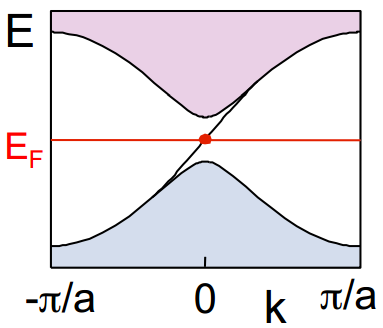
\includegraphics[width=0.5\linewidth]{diagrams/chiral_edge.png}
			\caption{Band insulator with chiral edge \footnotemark}
			%Not viewed as some integer number of orbitals filled per unit cell
		\end{figure}
		\begin{figure}
			\vskip-0.7cm
				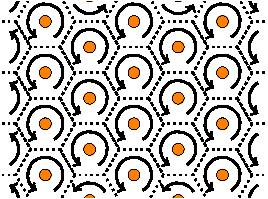
\includegraphics[width=0.5\linewidth]{diagrams/honeycomb_breakdown.pdf}
				\caption{}
		\end{figure}
\footnotetext[1]{
\citep{Hasan2010-fq}}		
}

\only<5>{
\begin{columns}[T]
	\begin{column}[T]{.5\textwidth}
		\begin{figure}
		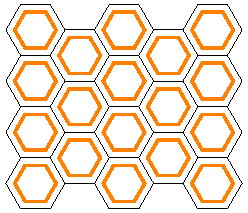
\includegraphics[width=.6\textwidth]{fbi3.pdf}
		\caption{Proposed Solution by \cite{kimchi2013}}
		\end{figure}
	\end{column}
	\begin{column}[T]{.5\textwidth}
					$$
\ket{\psi} = \prod\limits_{\varhexagon} \left(\sum\limits_{i \in \varhexagon} b^{\dagger}_i \right) \ket{\mathbf{0}}
			$$ 
	\end{column}
\end{columns}
}

'Classical cartoons and usual tricks' lead to symmetry breaking, as noticed by \cite{parameswaran2013}

\end{frame}
\begin{frame}[c]{Can we use `band bosons`?}
\vskip-1.5cm
\only<1>{
Band fermions have atomic insulator picture using Wannier functions.

$$W^{\alpha}_R(x) = \int_{B.Z.} d\kk e^{-iR\cdot \kk} \psi^{\alpha}_{\kk}(x)$$

$$d_R^{\alpha \dagger} = \sum\limits_x W^{\alpha}_R(x)c_x^{\dagger}$$ 

$$\ket{\psi} = \prod\limits_R d_R^{\alpha \dagger} \ket{\mathbf{0}} $$

Wannier functions are not unique and often don't respect lattice symmetries depending on choice of phase for original basis functions. 
\\\vspace{1em}
But the resulting 'Slater determinant' wavefunction is symmetric regardless. 
%due to antisymmetrization
%individual wannier functions are not eigenstates unless the band is perfectly flat.
%This picture breaks down when the chern number of a band is not zero, or if bands touch.
}
% A band boson is defined in analogy to this slater determinant wave
\only<2>{
\begin{block}{`Band bosons' a.k.a. Boson Permanent}
{A boson permanent wavefunction created from filling an orbital $\phi_{R+x}$ for each unit cell $R$ with a boson}
\end{block}
Analogous to the Slater determinant for fermions except:
%with a few key differences:
\bi 
\item $\ket{\psi}$ respects lattice symmetries only if $\phi$ does
%Boson permanent wavefunction won't respect lattice symmetries unless orbitals filled do.
\item $H$ needs repulsive interactions to stop Bose condensation
\bi 
\item e.g. $H_{BH}$ with $$d^{\dagger}_R = \sum\limits_i \phi_i b^{\dagger}_i$$
\ei
%use bose-hubbard repulsion
\item Orbitals will need to be localized and orthogonal for $H_{BH}$ to be a parent Hamiltonian
\ei 

%If we could find symmetric, orthogonal, localized orbitals, we can try fill them with bosons to make a 'band' boson featureless insulator with a nice parent Hamiltonian.
%Say by analyzing the fermion tightbinding model 
%Can do this on Kagome but not on honeycomb: the symmetry protection of the band touching is an obstruction
}
\end{frame}
\begin{frame}[c]{Honeycomb Featureless Boson Insulator}
\framesubtitle{Proposed Wavefunction}
\vskip-1.5cm
\only<1>{
\begin{figure}[h]
\scalebox{1}{
% y=\sqrt{3/4}*(minimum size)/2
%

%http://tex.stackexchange.com/questions/6019/drawing-hexagons
\begin{tikzpicture}[x=7.5mm,y=4.33mm]
  % some styles
  \tikzset{
    box/.style={
      regular polygon,
      regular polygon sides=6,
      minimum size=10mm,
      inner sep=0mm,
      outer sep=0mm,
      rotate=0,
     %dotted,
     thin,
      black,
      draw
    }
  }
  \tikzset{
    bbox/.style={
      regular polygon,
      regular polygon sides=6,
      minimum size=2mm,
      fill,
      inner sep=0mm,
      outer sep=0mm,
      rotate=0,
     % dotted,
     very thick,
     orange,
      draw
    }
  }
 \tikzset{boson/.style={circle=1pt,draw=black!100,fill=orange!100,inner sep=2pt}}
  \tikzset{dimer/.style={ellipse=1pt,draw=black!100,fill=orange!90,inner sep=2pt}}
    \tikzset{thindimer/.style={ellipse=1pt,draw=black!100,fill=orange!90,inner sep=1pt}}

\foreach \i in {0,...,2} 
    \foreach \j in {0,...,3} {
            \node[box] at (2*\i,2*\j) {};
        }
\foreach \i in {0,...,1} 
    \foreach \j in {0,...,2} {
   	   \node[box] at (2*\i+1,2*\j+1) {};   
        }
        
\foreach \i in {0,...,2} 
    \foreach \j in {0,...,3} {
            \node[bbox] at (2*\i,2*\j) {};
        }
\foreach \i in {0,...,1} 
    \foreach \j in {0,...,2} {
   	   \node[bbox] at (2*\i+1,2*\j+1) {};   
        }

\end{tikzpicture}
}
\end{figure}
}

\only<2>{
\begin{figure}[h]
\scalebox{1}{
% y=\sqrt{3/4}*(minimum size)/2
%

%http://tex.stackexchange.com/questions/6019/drawing-hexagons
\begin{tikzpicture}[x=7.5mm,y=4.33mm]
  % some styles
  \tikzset{
    box/.style={
      regular polygon,
      regular polygon sides=6,
      minimum size=10mm,
      inner sep=0mm,
      outer sep=0mm,
      rotate=0,
     %dotted,
     thin,
      black,
      draw
    }
  }
  \tikzset{
    bbox/.style={
      regular polygon,
      regular polygon sides=6,
      minimum size=4mm,
      %fill,
      inner sep=0mm,
      outer sep=0mm,
      rotate=0,
     % dotted,
     very thick,
     orange,
      draw
    }
  }
 \tikzset{boson/.style={circle=1pt,draw=black!100,fill=orange!100,inner sep=2pt}}
  \tikzset{dimer/.style={ellipse=1pt,draw=black!100,fill=orange!90,inner sep=2pt}}
    \tikzset{thindimer/.style={ellipse=1pt,draw=black!100,fill=orange!90,inner sep=1pt}}

\foreach \i in {0,...,2} 
    \foreach \j in {0,...,3} {
            \node[box] at (2*\i,2*\j) {};
        }
\foreach \i in {0,...,1} 
    \foreach \j in {0,...,2} {
   	   \node[box] at (2*\i+1,2*\j+1) {};   
        }
        
\foreach \i in {0,...,2} 
    \foreach \j in {0,...,3} {
            \node[bbox] at (2*\i,2*\j) {};
        }
\foreach \i in {0,...,1} 
    \foreach \j in {0,...,2} {
   	   \node[bbox] at (2*\i+1,2*\j+1) {};   
        }

\end{tikzpicture}
}
\end{figure}
}

\only<3>{
\begin{figure}[h]
\scalebox{1}{
% y=\sqrt{3/4}*(minimum size)/2
%

%http://tex.stackexchange.com/questions/6019/drawing-hexagons
\begin{tikzpicture}[x=7.5mm,y=4.33mm]
  % some styles
  \tikzset{
    box/.style={
      regular polygon,
      regular polygon sides=6,
      minimum size=10mm,
      inner sep=0mm,
      outer sep=0mm,
      rotate=0,
     %dotted,
     thin,
      black,
      draw
    }
  }
  \tikzset{
    bbox/.style={
      regular polygon,
      regular polygon sides=6,
      minimum size=7mm,
      %fill,
      inner sep=0mm,
      outer sep=0mm,
      rotate=0,
     % dotted,
     very thick,
     orange,
      draw
    }
  }
 \tikzset{boson/.style={circle=1pt,draw=black!100,fill=orange!100,inner sep=2pt}}
  \tikzset{dimer/.style={ellipse=1pt,draw=black!100,fill=orange!90,inner sep=2pt}}
    \tikzset{thindimer/.style={ellipse=1pt,draw=black!100,fill=orange!90,inner sep=1pt}}

\foreach \i in {0,...,2} 
    \foreach \j in {0,...,3} {
            \node[box] at (2*\i,2*\j) {};
        }
\foreach \i in {0,...,1} 
    \foreach \j in {0,...,2} {
   	   \node[box] at (2*\i+1,2*\j+1) {};   
        }
        
\foreach \i in {0,...,2} 
    \foreach \j in {0,...,3} {
            \node[bbox] at (2*\i,2*\j) {};
        }
\foreach \i in {0,...,1} 
    \foreach \j in {0,...,2} {
   	   \node[bbox] at (2*\i+1,2*\j+1) {};   
        }

\end{tikzpicture}
}
\end{figure}
}

\only<4->{
\begin{figure}[h]
\scalebox{1}{
\documentclass[twocolumn,english,prb,showpacs]{revtex4-1}
\usepackage[colorlinks=true,urlcolor=blue,citecolor=blue,linkcolor=blue]{hyperref}
\usepackage[T1]{fontenc}
\usepackage[latin9]{inputenc}
\usepackage{amssymb}
\usepackage{graphicx}
\usepackage{amsmath,color}
\usepackage{mathrsfs}
\usepackage{float}
\usepackage{indentfirst}
\usepackage{babel}
\usepackage[sort&compress]{natbib}
\usepackage{color}

\newcommand{\bela}[1]{[\emph{\color{blue}{Bela: #1}}]}
\newcommand{\brayden}[1]{[\emph{\color{red}{Brayden: #1}}]}
\newcommand{\eqnref}[1]{Eq.~(\ref{#1})}

%\makeatletter

%%%%%%%%%%%%%%%%%%%%%%%%%%%%%%
%These may need modification
%\usepackage[section]{placeins}
\graphicspath{{../images/}{../diagrams/}{.}} %what folders to look for images in, via the command \includegraphics
\newcommand{\beq}{\begin{equation}}
\newcommand{\eeq}{\end{equation}}
\newcommand{\beqa}{\begin{eqnarray}}
\newcommand{\eeqa}{\end{eqnarray}}
\newcommand{\bi}{\begin{itemize}}
\newcommand{\ei}{\end{itemize}}
\newcommand{\ket} [1] {\vert #1 \rangle}
\newcommand{\bra} [1] {\langle #1 \vert}
\newcommand{\braket}[2]{\langle #1 | #2 \rangle}
\newcommand{\ev}[1]{\langle #1 \rangle}
\newcommand{\vbra}[1]{\left ( #1 \right |}
\newcommand{\vket}[1]{\left |#1 \right )}
\newcommand{\vbraket}[2]{\left ( #1 \middle |#2 \right )} 
\newcommand{\braopket}[3]{\left \langle #1 \middle |#2 \middle | #3 \right \rangle} 
\newcommand{\vbraopket}[3]{\left ( #1 \middle |#2 \middle | #3 \right )} 

%\newcommand<>{\highlighton}[1]{%
%  \alt#2{\structure{#1}}{{#1}}
%}

\newcommand{\icon}[1]{\pgfimage[height=1em]{#1}}

\usepackage{empheq}

\newlength\mytemplen
\newsavebox\mytempbox

\makeatletter
\newcommand\mybluebox{%
    \@ifnextchar[%]
       {\@mybluebox}%
       {\@mybluebox[0pt]}}

\def\@mybluebox[#1]{%
    \@ifnextchar[%]
       {\@@mybluebox[#1]}%
       {\@@mybluebox[#1][0pt]}}

\def\@@mybluebox[#1][#2]#3{
    \sbox\mytempbox{#3}%
    \mytemplen\ht\mytempbox
    \advance\mytemplen #1\relax
    \ht\mytempbox\mytemplen
    \mytemplen\dp\mytempbox
    \advance\mytemplen #2\relax
    \dp\mytempbox\mytemplen
    \fcolorbox{airlightblue}{white}{\hspace{1em}\usebox{\mytempbox}\hspace{1em}}}

\makeatother

%\usepackage{wasysym}
\usepackage{amsfonts}
\usepackage{booktabs}
%%%%%%%%%%%%%%%%%%%%%%%%%%%%%%%

\begin{document}

\title{Not so featureless after all: symmetry protected order in an interacting boson state}

\author{Brayden Ware}
\affiliation{Department of Physics, University of California, Santa Barbara, CA, 93106-6105, USA}

\author{Itamar Kimchi}
\affiliation{Department of Physics, University of California, Berkeley, CA 94720, USA}

\author{S. A. Parameswaran}
\affiliation{Department of Physics and Astronomy, University of California, Irvine, CA 92697, USA}

\author{Bela Bauer}
\affiliation{Station Q, Microsoft Research, Santa Barbara, CA 93106-6105, USA}

\begin{abstract}
While the Lieb-Schultz-Mattis theorem forbids the existence of fully symmetric quantum paramagnetic phases on lattices with fractional filling of particles per unit cell, such a phase is in principle allowed with certain fractional numbers of particles per site on non-Bravais lattices, including half-filling on the honeycomb lattice. It has been shown that a non-interacting Hamiltonian of spinless fermions or bosons cannot have such a symmetric insulating ground state, and an explicit construction using interactions is challenging. Recently, Kimchi et al. constructed a wavefunction for bosons at half-filling that does not break any symmetries and is not topologically ordered--and in this sense is a featureless insulator in the bulk. Here, however, we reveal that this wavefunction exhibits non-trivial structure at the edge. We apply recently developed techniques based on a tensor network representation of the wavefunction to demonstrate the presence of a gapless entanglement spectrum and a non-trivial action of combined charge-conservation and spatial symmetries on the edge. We will also discuss the possibility of finding a parent Hamiltonian and analyzing the existence of a symmetry-protected topological phase around this state.
\end{abstract}
\maketitle

%!TEX root = ../fbi.tex

\section{Introduction}


Featureless insulator problem description from   \onlinecite{parameswaran2013}
\bi 
\item Classical Mott insulators have integer site filling
\item LSM forbids featureless insulators at fractional unit cell 
filling. Site-filling can still be multiples of $1/n$
\item Extensions to LSM in \onlinecite{parameswaran2013-2} further 
forbid some site fractional site fillings for non-symmorphic lattices.
\ei 

In addition to finding featureless states, we also want to determine
 if different featureless states are in the same phase, i.e. whether 
 they can be connected without a phase transtion, but while preserving 
 the symmetry of the Hamiltonian H. Of particular interest are those 
 featureless states that cannot be connected adiabatically to a 
 product state without breaking the symmetry; these are called 
 symmetry protected topological (SPT) phases. Instead of local order 
 parameters, the distinguishing "features" of these phases appear at 
 phase boundaries, such as the edge of an open system, and in 
 entanglement properties of the bulk wavefunction.



 connecting path of Hamiltonians with featureless ground states everywhere along the path. Since the ground state degeneracy on a torus changes

SPT phases for a symmetry group G are featureless states 

The simplest example of a tensor network for a 1D system is a matrix 
product state; translationally-invariant matrix product states (MPS) 
are represented by a single rank 3 tensor $A_p^{ij}$ which specifies 
the wavefunction coefficients in a given basis local basis as a 
product of matrices $$\ket{\psi} = \sum\limits_{\{p_i\}} A_{p_1} 
A_{p_2} ... A_{p_N} \ket{p_0 p_1 ... p_N},$$ with one matrix for each 
site in the one-dimensional system.

PEPS are the generalization of MPS to two and higher dimensions, where 
each site in the system is represented by a rank $z+1$ tensor, where 
$z$ is the coordination number of the lattice, and wavefunction 
coefficients are similarly given by contracting over all virtual 
indices as shown in Figure \ref{fig:PEPS}.\cite{verstraete2004}

\section{F.B.I. wavefunction}

...\cite{Kimchi2012-lr}

\section{PEPS Construction of honeycomb F.B.I.}
\begin{figure}[H]
	\centering
	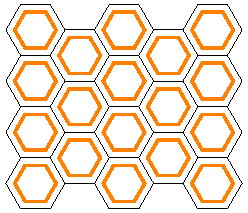
\includegraphics[width=0.6\columnwidth]{fbi3.pdf}
\end{figure}

\begin{figure}[H]
	\centering
	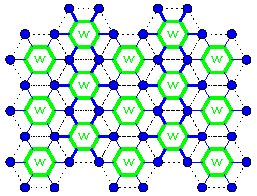
\includegraphics[width=0.6\columnwidth]{FI_PEPS.pdf}
\end{figure}

\begin{figure}[H]
	\centering
	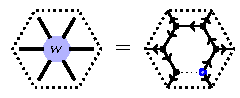
\includegraphics[width=0.6\columnwidth]{w_string.pdf}
\end{figure}

\begin{figure}[H]
	\centering
	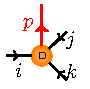
\includegraphics[width=0.3\columnwidth]{D_op.pdf}
\end{figure}
%!TEX root = ../fbi.tex

\section{Entanglement spectrum}
\label{sec:ES}

The quasi-1D cylinder geometry is also convenient for calculating the entanglement spectrum for 
entanglement cuts transverse to the cylinder. The procedure for computing the Schmidt decomposition is the 
same as for a MPS, and implies a canonical form for the quasi-1D MPS

$$
\ket{\psi} = \sum\limits_{\{p_i\}} \Gamma_{p_1} \Lambda \Gamma_{p_2} ... \Lambda \Gamma_{p_N} \ket{p_0 p_1 ... p_N}.
$$

The elements $\lambda_i$ of the diagonal matrix $\Lambda$ which appears in the canonical form,
are related to the non-zero eigenvalues $\rho_i$ of the reduced density matrix for the left or right half
of the system via $\rho_i = \lambda_i^2$.

The entanglement spectrum $\epsilon_i$  is defined via the equation $e^{-\epsilon_i} = \rho_i$. One says that the entanglement spectrum



Briefly discuss how the entanglement spectrum is calculated.\cite{cirac2011}

The entanglement spectrum shows a linear dispersion near momentum zero. Many points in the spectrum are 
doubly degenerate - those that are assigned a non-zero $U(1)$ charge.
	
\begin{figure}[H]
	\centering
	\includegraphics[width=\columnwidth]{{EntanglementSpectrum_L10.pdf}}
	\caption{Entanglement spectrum on a zig-zag edge L=10 cylinder}
	\label{fig:ESL10}
\end{figure}

On odd circumference cylinders, the entire entanglement spectrum is doubly degenerate.

\begin{figure}[H]
	\centering
	\includegraphics[width=\columnwidth]{{EntanglementSpectrum_L9.pdf}}
	\caption{Entanglement spectrum on a zig-zag edge L=9 cylinder}
	\label{fig:ESL9}
\end{figure}

The topological entanglement entropy is essentially zero.

\begin{figure}[hbctp]
	\centering
	\includegraphics[width=\columnwidth]{{TopologicalEntanglementEntropy.pdf}}
	\caption{The topological entanglement entropy $\gamma$ is consistent with 0.}
\end{figure}

The entanglement gap closes roughly as $1/L$. 

\begin{figure}[H]
	\centering
	\includegraphics[width=\columnwidth]{{EntanglementEnergyScaling.pdf}}
  \caption{Power law fits for the lowest five states above the ground state in Figure \ref{fig:ESL10}. The 
  $1/L$ scaling is a signature of a gapless (entanglement) Hamiltonian. Due to the small system size, 
  points at non-zero momentum still deviate significantly from $1/L$ scaling.}
\end{figure}

\newcommand{\uL}{\mathbf{L_0}}
\newcommand{\bL}{\mathbf{\bar{L}_0}}

\subsection{Identification of edge CFT}

Given the $U(1)$ symmetry of the state, the simplest possible conformal field theory we might expect to 
appear at the edge is that of a single free bosonic field. 

The free-boson CFT is created from the Lagrangian 
$$ \mathfrak{L} = \frac{g}{2}\int dt \int\limits_0^L dx ( \frac{1}{v^2}(\partial_t \phi)^2 - (\partial_x \phi)^2)$$
and with the compatified field identification
$$ \phi \equiv \phi + 2\pi R$$
and placed on the circle of circumference $L$ with periodic boundary conditions
$$ \phi(x) \equiv \phi(x+L).$$

After canonical quantization, it is found that the set of energy eigenstates consists of $U(1)$ Kac-Moody 
primaries $\ket{e, m}$, with integers $e, m$ labeling the $U(1)$ charge and the winding number of the 
bosonic field respectively, and level $n, \bar{n}$ descendant fields for each primary - such as  
$\mathbf{\bar{j}}_{-\bar{n}} \mathbf{j}_{-n} \ket{e, m}$ - for any nonnegative integers $n, \bar{n}$. The 
number of level $n, \bar{n}$ descendants of a given primary, all of which are degenerate, is $Z(n) 
Z(\bar{n})$, where $Z(n)$ is the number of partitions of the integer $n$.

The properties of the $U(1)$ Kac-Moody algebras constrain the form of energy and momentum eigenvalues - 
for the state $\mathbf{\bar{j}}_{-\bar{n}} \mathbf{j}_{-n} \ket{e, m}$, 

\begin{align*}
	\mathbf{P} =\frac{2\pi}{L}&(\uL-\bL) 
	&=& \frac{2\pi}{L}(em + n - \bar{n}) \\
	\mathbf{H} = \frac{2\pi}{L}&(\uL+\bL) 
	&=& \frac{2\pi}{L}(\frac{\kappa e^2}{2} + \frac{m^2}{2 \kappa} + \frac{n + \bar{n}}{2}) %\\
\end{align*}

By rescaling the energy and momentum, we find a system size independent pattern that can be matched to the 
low-energy, linearly dispersing part of the entanglement spectrum from Figures \ref{fig:ESL10} and 
\ref{fig:ESL9}. 

\begin{align*}
\mathbf{P} &\propto (em + n - \bar{n}) \\
\mathbf{H} &\propto e^2 + \frac{m^2}{\kappa^2} + \frac{1}{\kappa}(n + \bar{n})
\end{align*}

The label $m$ is 0 for all states in the linearly dispersing cone around $K=0$ - however, the primary 
states $\ket{e, m=\pm 1}$ can be found centered around momentum $K=\pi$, as seen in critical spin chains 
[reference]. The states with nonzero $e$ and zero $m$ are degenerate in energy and momentum with the same 
state with charge $-e$, but the $Z(n)Z(\bar{n})$ degeneracies predicted for descendant states are split by 
finite size effects.

The parameter $\kappa$ that appears - related to the coupling constant $g$ in the effective Lagrangian - 
is free. Quantum models that exhibit critical points that show the behavior of the free-boson CFT in fact 
have a whole line of critical points with varying values of $\kappa$, which can be tuned using a marginal 
operator in the theory.

\begin{figure}[H]
	\centering
	\includegraphics[width=\columnwidth]{EEIdentify.pdf}
	\caption{The identification of the primary states $\ket{\pm e, m=0}$ and the level $n, \bar{n}$ 
	descendants in the spectrum of the soft-core boson entanglement Hamiltonian. The states are labeled 
	$e_{n, \bar{n}}$. The zero and scale of the numerical spectrum are set by matching the lowest two 
	states. The energies and charges of the primaries with charges $2, 5/2, ... 4$ appear at the predicted 
	spots.  The best estimate for the Luttinger parameter from this spectrum is $\kappa \approx 1/6.4$, 
	taken from the energy of the $0_{1, 0}$ state. }
\end{figure}

We can also take the lowest-lying Schmidt state, interpret it as the ground state of a 1d Hamiltonian, and 
consider its entanglement.

\begin{figure}[H]
	\centering
	\includegraphics[width=\columnwidth]{{EdgeGS_EntanglementEntropy.pdf}}
	\caption{Entanglement entropy within the entanglement ground state of the soft-core boson state on $10$ 
	sites. For 	    comparison, the Cardy-Calabrese formula $S(x) = c/3 \log \sin( \pi x/L) + const.$ is 
	shown with $c=\frac{1}{2}, 1,$ and $2$, with the $const.$ fixed by matching the maximum of the 
	entanglement entropy data. $c=1$ is a good fit.}
	\label{fig:EdgeGS_EE}
\end{figure}



\subsection{Symmetry action on the edge}

\begin{figure}[H]
    \centering
    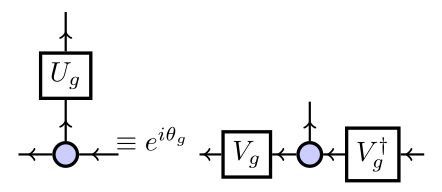
\includegraphics[width=0.6\columnwidth]{group_sym.png}
\end{figure}


\begin{figure}[H]
    \centering
    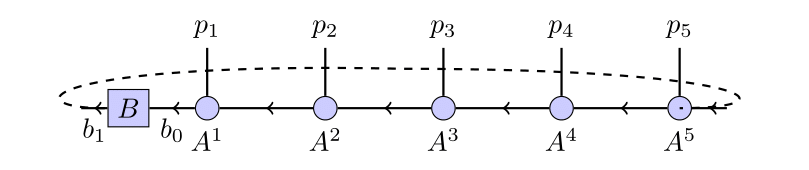
\includegraphics[width=\columnwidth]{mpsbc.png}
\end{figure}

\begin{tabular*}{\columnwidth}{@{\extracolsep{\stretch{1}}}*{5}{r}@{}}
\toprule
$\mathbf{G}$ & $\mathbf{U_g}$ & $\mathbf{\theta_g}$ & $\mathbf{V_g}$ &$\mathbf{V_g V^*_g}$ \\
\midrule
 $U(1)$ & & & & \\
 $\mathcal{\pi}$ & & & & \\
 $\mathcal{I}$ & & & & \\
 $\mathcal{\pi} \mathcal{I}$ & & & & \\
\bottomrule
\end{tabular*}

Since 
$$  
V_{\mathcal{\pi} \mathcal{I}} V_{\mathcal{\pi} \mathcal{I}}^* = -I \text{\quad or \quad } V_{\mathcal{\pi}} V_{\mathcal{I}} = - V_{\mathcal{I}} V_{\mathcal{\pi}},
$$ 

the representation is in the nontrivial class of 

$$
H^2(\mathbb{Z}_2 \times \mathbb{Z}_2^{\mathcal{I}}; U(1)) = \mathbb{Z}_2.
$$

\section{Identification of edge CFT}

\section{Symmetry protected topological order}
%!TEX root = ../fbi.tex

\section{Conclusion and Discussion}

\appendix

\section{Determining the edge action of the symmetry using MPS}
\label{Appendix:MPS}

We can use the formalism of MPS to assign an action
of the symmetry on the Schmidt states, and in particular for the charge and 
translation on-site symmetries the Schmidt states can be simultaneously assigned
charge and translation quantum numbers. This method of discovering the symmetry 
action will reproduce the action discussed in \ref{sec:ES} and quantum numbers used
in the spectra plots shown in Fig.~\ref{fig:ESL910}.
  
Let's discuss this formalism briefly. In addition,
we will discuss a generalization of this method that allows us to numerically
determine the symmetry action of inversion symmetry on the Schmidt states,
as in Section~\ref{sec:symmetry}. 
Both of these discussions follow Ref.~\onlinecite{pollmann2010}.

These discussions start by finding tensors $\Gamma, \Lambda$ representing the 
so-called canonical form of the MPS, as
originally detailed in \cite{perezgarcia2008}. This canonical form provides the Schmidt
decomposition at each site in the lattice.
\beq
\ket{\psi} = \sum\limits_{\{p_i\}} \ldots \Lambda \Gamma_{p_0} \Lambda \Gamma_{p_1} \Lambda \Gamma_{p_2} \Lambda \ldots \ket{... p_0 p_1 p_2 ...}.
\eeq
As a reminder, each physical leg represents all $2W$ physical sites on a cylinder slice,
and each virtual leg represents all virtual indices that connect cylinder slices.
The change of basis to canonical form generally mixes the Hilbert spaces from these
virtual legs, so the resulting basis won't be local around the circumference
of the cylinder.

Each on-site symmetry of the wavefunction $U_g = \otimes_i u^i_g$, with $U_g
\ket{\psi} = e^{i \Theta_g} \ket{\psi}$ is assigned an operator $V_g$ that
acts on the virtual leg of the MPS, that satisfies the equation
\begin{center}
\beq
\label{eq:onsitesym}
\eeq
\vskip-5em
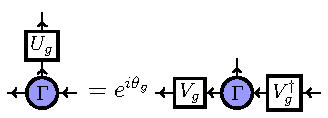
\includegraphics[width=0.6\columnwidth]{group_sym.pdf}.
\end{center}
This equation can be rewritten and solved as an eigenvector problem;
for an MPS with a nondegenerate largest transfer matrix eigenvalue,
this equation is guaranteed have a unique solution where the eigenvalue $e^{i \theta_g}$
is the largest eigenvalue of the eigenvector problem.

The solutions $V_g$ have two important properties: they are only defined up to a phase,
and they are guaranteed to commute with the diagonal matrix $\Lambda$ of Schmidt weights.  

Due to the first property, these operators are not guaranteed to form a linear
representation of the group of on-site symmetries, but in general could make
up a projective representation, satisfying
$$V_g V_h = e^{i \omega(g, h)} V_{gh}.$$ 
It is not always possible to absorb these phases into the definitions of the $V_g$.
The set of equivalent classes of phases $\omega(g, h)$ 
under redefinitions $V_g \to \alpha(g)V_g$ is called $H^2(G, U(1))$, the second group 
cohomology with $U(1)$ coefficients. 

For all the groups discussed in this paper, the group cohomology classes are labeled by
elements of a discrete abelian group - these discrete classes cannot be connected to each other
continuously. Physically, only a phase transition or breaking the symmetry allows one to connect
the different projective symmetry actions. 
Additionally, the classification of projective representations for the on-site symmetry group 
$U(1) \times \mathbb{Z}_W$ representing charge and translation around the cylinder is trivial. 
Thus, these edge symmetries can be taken to act linearly, 
and all Schmidt states can always be simultaneously assigned charge and momentum eigenvalues,
as in Figure~\ref{fig:ESL910}.

The second property guarantees that the $V_g$ only mixes exactly degenerate Schmidt states.
The action of $V_g$ must have the same phases $\omega(g, h)$ on each degenerate block of Schmidt 
states, so the projective representation can be nontrivial on any block only if every Schmidt 
state throughout the entire spectrum is degenerate. The degeneracy will be protected by the 
symmetry if and only if the $V_g$ form a nontrivial projective representation. Therefore
this 1D SPT analysis can only potentially give a nontrival answer for the odd $W$ states 
of the HFBI, where this exact degeneracy is seen throughout the spectrum. Nonetheless, we find 
there are no on-site symmetries of the wavefunction that can be used to explain the degenerate
entanglement spectrum of the odd $W$ HFBI states. Instead we must use an inversion symmetry. 

The MPS analysis of inversion symmetry works similarly. We will consider in general any symmetry  
$h$ of the wavefunction that squares to the identity and that can be written in the MPS as the 
product of an on-site symmetry action $U_h$ and a transpose of the site tensor.
This will include an inversion of the honeycomb lattice - equivalent to a 180 degree rotation 
about the center of any plaquette, which we label $\I = \I_y \I_x$, and the combination of
inversion with on-site symmetries. In addition, by blocking two site-tensors together, we
can write the reflection symmetry $\I_y$ in this form as well. In this scenario, the 
edge symmetry action satisfies
\begin{center}
\beq
\label{eq:onsitesym}
\eeq
\vskip-5em
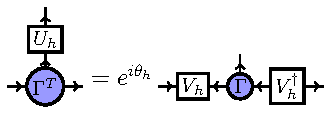
\includegraphics[width=0.6\columnwidth]{inv_sym.pdf}.
\end{center}
The map $V_{h}$ is also computed as a dominant eigenvector. 

For the HFBI, the symmetry group respected by the cylinder geometry is
$U(1) \times (\mathbb{Z}_W \rtimes \mathbb{Z}_2)
\times \mathbb{Z}_2^P \times \mathbb{Z}_2^T$, where the factors refer to charge
symmetry, translation around the cylinder, $\I_x$, $\I_y$, and $\tau$ respectively.
The $P$ and $T$ denote space-reversing and time-reversing symmetries, and signify the 
antiunitary action on the Schmidt states. 
%Compute the cohomology class of 
%$H^2(U(1) \times (\mathbb{Z}_W \rtimes \mathbb{Z}_2)
%\times \mathbb{Z}_2^P \times \mathbb{Z}_2^T ; U(1)) ?$
Many of the non-trivial projective
representations of such a complicated group will remain projective when the symmetry is
restricted to a subgroup - in this case, the full symmetry is not needed to protect the 
entanglement degeneracy. As shown in Table~\ref{table:sym}, the projective representation 
corresponding to the HFBI state can indeed be protected by any one of a number of subgroups 
of the full symmetry group, all involving inversions and charge parity.

The symmetry actions - both on-site and inversion symmetries -
are computed in the Schmidt basis, but can be transformed
into the basis $\vket{\{\sigma_i\}}$ determined by the virtual legs of the PEPS in
Figure~\ref{fig:FBI_PEPS_2}. 
In this case, the symmetry action $V_{\I_y}$ is precisely
a particle-hole symmetry in the local PEPS basis, with coefficients
$$
V_{\I_y}\vket{\sigma_1, \ldots, \sigma_{W}} = \vket{1-\sigma_1, \ldots, 1-\sigma_{W}}, 
$$
since a state where the $i^{th}$ hexagon contributes $\sigma_i$ bosons on the right is paired with
a state where the $i^{th}$ hexagon contributes $1-\sigma_i$ on the left.
Thus 
$$
V_{\I_y} = \prod\limits_i \sigma_i^x K,
$$
where K is complex conjugation in the local PEPS basis, and $\sigma_i^x$ is the Pauli
operator acting on the $i^{th}$ site of the local PEPS basis.

Charge symmetry acts locally as well:
$$
e^{i \theta \mathcal{Q}}\vket{\sigma_1, \ldots, \sigma_{W}} = e^{i \theta \sum(\sigma_i-1/2)}\vket{\sigma_1, \ldots, \sigma_{W}}.
$$
In particular, charge parity $V_{\varPi} = e^{i \theta \mathcal{Q}}$ can be written as
$$V_{\varPi} = e^{i \pi \sum(\sigma_i - 1/2)} = \prod\limits_i \sigma_i^z.$$

The combined action of charge parity and reflection across the cut takes the form 
$$
V_{\varPi \I_y} = \prod\limits_i \left(i \sigma_i^y \right) K,
$$
which is precisely the form that time-reversal acting on an ordinary spin-$\frac12$ chain takes.
When the circumference of the cylinder $W$ is odd, we see that
$$V_{\varPi \I_y}V_{\varPi \I_y}^{*} = -I.$$ 
The degeneracy of the entanglement spectrum can be seen as an application of Kramer's theorem.
Formally, this property is said to characterize the nontrivial projective representation
$$
H^2(\mathbb{Z}_2^P; U(1)) = \mathbb{Z}_2,
$$
and remains true while $\varPi \I_y$ is a symmetry and no phase transitions have occurred.

Time reversal symmetry acts as complex conjugation in the local PEPS basis $V_{\tau}=K$.
Translation and $\I_x$ act as permutations of the local PEPS basis:
\begin{equation*}
\begin{split}
V_{T}\vket{\sigma_1, \ldots, \sigma_{W}} &= \vket{\sigma_2, \ldots, \sigma_{W}, \sigma_{1}} \\
V_{\I_x}\vket{\sigma_1, \ldots, \sigma_{W}} &= \vket{\sigma_W, \ldots, \sigma_{1}}.
\end{split}
\end{equation*}
These symmetries can be combined with $V_{\varPi \I_y}$ to create the additional topological 
invariants shown in Table~\ref{table:sym}. A non-trivial projective 
representation in $$H^2(\mathbb{Z}_2 \times \mathbb{Z}_2; U(1)) = \mathbb{Z}_2$$
is created whenever two unitary symmetries that commute in the bulk satisfy 
$$V_{g_1} V_{g_2} V_{g_1}^{-1} V_{g_2}^{-1} = -I.$$
Each new invariant is related to a new set of pertubations that can't break the entanglement 
degeneracy. 

\section{Local Hamiltonian for the Edge free boson CFT}
\label{Appendix:LocalEdge}

B

\section{Mode expansion and symmetry action of free-boson CFT}
\label{Appendix:CFT}
How do the symmetry protecting operations act on the CFT states
$\ket{e, m, \{n_i\}, \{\bar{n}_i\}}$?

From that, infer how they act on the free boson fields $\phi$ and $\theta$.

Which perturbations to the CFT gap it out completely or spontaneously break the symmetry?

Are those pertubations forbidden by the implementation of symmetry on the edge.

\section{Variants on the HFBI wavefunction}
\subsection{Tuning soft-core bosons to hard-core}
In Equations~\eqref{eqn:Dsc} and \eqref{eqn:Dhc}, the tensor $D$ can be replaced by a more general form 
\begin{equation} \label{eqn:Dgen}
D_{p, i_0 i_1 i_2}  = \left\{ \begin{array}{ll}
													d_p  &: p =i_0+i_1+i_2  \\
													0  &:  \text{else}
													\end{array}
											\right. ,
\end{equation}
which the coefficients $d_p = 1,\, 1,\, \sqrt{2},\,\sqrt{6}$ for $p = 0,\, 1,\, 2,\, 3$ in the soft-core state and $d_p = 1,\, 1,\, 0,\, 0$ for $p = 0,\, 1,\, 2,\, 3$ in the hard-core state. We can continously tune the coefficients $d_2$ and $d_3$ from the soft-core to the hard-core values.
Upon doing so, we find that the transfer matrix spectrum remains gapped, with the correlation length monotonically increasing from the soft-core state to the hard-core state. 
Furthermore, the low energy parts of the entanglement spectrum do not change significantly through this tuning.
Therefore we expect that the hard-core and soft-core phases can be adiabatically connected with a 
path of local Hamiltonians, and all SPT results that apply to one state apply to the other. By choosing appropriate values of $d_2$ and $d_3$, we can also make replace the vacuum $\ket{0}$ in
Equation~\eqref{eq:def} with a constant background of $N$ filled bosons $\ket{N}$, or even make
states of spins $S$ where Equation~\eqref{eq:def} becomes
\begin{equation} \label{eq:spindef}
\ket{\psi} = \prod\limits_{\varhexagon} \left( \sum\limits_{i \in \varhexagon} S^{+}_{i} \right) \ket{S_z = m}.
\end{equation}

\subsection{Inversion Protected Phase}
Additionally, the tensor $W$ in Equation~\eqref{eq:W} can be replaced by the more general form
\begin{equation} \label{eq:Wgen}
W^{n_1 \ldots n_6}  = \left\{ \begin{array}{lr}
													p_x  : & n_x=1,\, n_y = 0
													\; \forall \; y \neq x \\
													0  : & \text{else}
													\end{array} \right.,
\end{equation}
which corresponds to modifying Equation~\eqref{eq:def} to 
\begin{equation} \label{eq:pdef}
\ket{\psi_{\ell}} = \prod\limits_{\varhexagon} \left( \sum\limits_{i \in \varhexagon} p_i b^{\dagger}_{i} \right) \ket{0}.
\end{equation}

This does not in general preserve the rotational symmetry of the state, but it does if the 
coefficients $p_0, \ldots p_5$ are in an angular momentum mode $$p_x = e^{i x \ell}$$ where
$\ell \in \{0, 2\pi/6, \ldots 5\pi/6 \}$. These 6 discrete solutions can't be continously tuned to one another while preserving all the lattice symmetries.

The state $\ket{\psi_{\ell=\pi}}$ can be shown to be related to state $\ket{\psi_{\ell=0}}$ discussed in the main text by a on-site unitary operator $U(\pi)$, 
where 
\begin{equation} \label{eq:Uphi}
U(\varphi) = \prod\limits_{j \in B} e^{i \varphi \hat{Q}_j}.
\end{equation}
Due to this relation, $\ket{\psi_{\ell=\pi}}$ and $\ket{\psi_{\ell=0}}$ have identical correlation lengths and entanglement spectra. 
However, the protecting symmetries from Table~\ref{table:sym} are mapped using conjugation
by $U(\pi)$ into a new set of protecting symmetries, shown in Table~\ref{table:pisym}. 

\begin{table}
\begin{tabular*}{\columnwidth}{@{\extracolsep{\stretch{1}}}*{4}{r}@{}}
\toprule
Group & Generators & Invariant & $i$  \\
\midrule
$\mathbb{Z}_2^P$ & $\{\I \}$ 
& $V_{\I} V_{\I}^* = -I$ &$-$ \\
$\mathbb{Z}_2^P$ & $\{\I_y \}$ 
&$V_{\I_y} V_{\I_y}^* = -I$ &$-$ \\ \hline
$\mathbb{Z}_2 \times \mathbb{Z}_2^{PT}$& $\{\varPi, \tau \varPi \I\}$ 
&$V_{\varPi} V_{\tau \varPi \I} V_{\varPi}^{-1} V_{\tau \varPi \I}^{-1} = -I$ &$+$ \\
$\mathbb{Z}_2 \times \mathbb{Z}_2^{PT}$& $\{\varPi, \tau \varPi \I_y\}$
&$V_{\varPi} V_{\tau \varPi \I_y} V_{\varPi}^{-1} V_{\tau \varPi \I_y}^{-1} = -I$ &$+$ \\
$\mathbb{Z}_2 \times \mathbb{Z}_2^{PT}$& $\{\varPi \I_x, \tau \varPi \I\}$
&$V_{\varPi \I_x} V_{\tau \varPi \I} V_{\varPi \I_x}^{-1} V_{\tau \varPi \I}^{-1} = -I$&$+$ \\
$\mathbb{Z}_2 \times \mathbb{Z}_2^{PT}$& $\{\varPi \I_x, \tau \varPi \I_y\}$
&$V_{\varPi \I_x} V_{\tau \varPi \I_y} V_{\varPi \I_x}^{-1} V_{\tau \varPi \I_y}^{-1} = -I$ &$+$\\
\bottomrule
\end{tabular*}
\caption{Summary of symmetry protecting invariants found for the $\ket{\psi_{\ell=\pi}}$ state. 
The degenerate entanglement spectrum cannot be split unless all 6 of the  minimal protecting symmetry groups are broken. }
\label{table:pisym}
\end{table}

Notably,
since
$$
U(\pi) \varPi \I U(\pi)^{\dagger} = \I, 
$$
this state has doubly degenerate entanglement spectra on odd cylinder sizes protected by lattice inversion symmetry alone.

A similar mapping for 1-D inversion protected states is discussed in Appendix A of Ref.~\onlinecite{pollmann2010}. As discussed \brayden{somewhere}, the state $\ket{\psi_{\ell=0}}$
on the $W=1$ cylinder is adiabatically connected to the 1-D Haldane insulator state discussed in
Ref.~\onlinecite{pollmann2010}. The new $\ket{\psi_{\ell=\pi}}$ state on the $W=1$ cylinder is instead adiabatically connected to the 1-D AKLT state. 

\label{Appendix:Variants}

\acknowledgements


\bibliography{fbi}


\end{document}

}
\end{figure}
}
\end{frame}
\begin{frame}{Goals for Honeycomb Mott Insulator}
\vskip-1.5cm
\bi 
\item Build a tensor network representation for doing computations
\item <1-> Verify that no spontaneous symmetry breaking occurs
%We'll do this by computing correlation functions on a cylinder geometry combined with scaling analysis in the circumference

\only<1>{
\begin{figure}
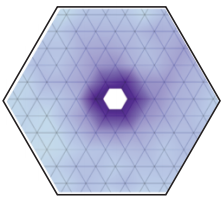
\includegraphics[width=6cm]{diagrams/kimchicorr.png}
\caption{Exponentially decaying rotationally symmetric correlations computed using Monte Carlo sampling, \citep{Kimchi2012-lr}}
\end{figure}
}

\only<2->{
\begin{figure}
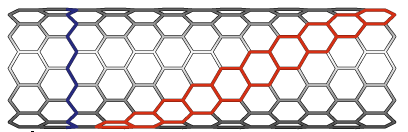
\includegraphics[width=6cm]{diagrams/Zig.png}
\end{figure}

\item<3-> Rule out topological order

\item<4-> Compute entanglement spectrum to check for nontrivial entanglement
\item<5-> Understand the role of symmetries in protecting entanglement in interacting quasi-1D and 2D theories
\item<6-> Find distinguishing topological invariant and/or physical signatures
\item<7-> Find a parent Hamiltonian 
%then you can do things like perturb hamiltonian to show that it is a stable phase if certain symmetries are kept, and drive phase transitions to lattice SB insulators or superfluids.
% also you can dope it and make a superfluid with some properties.

}
\ei 
\end{frame}

\section{Entanglement}
\begin{frame}{What is entanglement?}
\vskip-1.5cm
 When a wavefunction in a product Hilbert space cannot be written as a product state, it is \textbf{entangled}.
\only<1-2>{ 
\begin{block}{}
\begin{columns}[T]
    \begin{column}{.5\textwidth}
    $$
    \ket{\psi} = \ket{\psi_L} \otimes \ket{\psi_R} ?
    $$
    \end{column}
    \begin{column}[T]{.5\textwidth}
        \only<1>{
        \note{A state in a product Hilbert space is a tensor}
        \vskip-1.5cm
        \begin{figure}
        \scalebox{0.8}
        {
        %!TEX root = ../thesis.tex

%\beginpgfgraphicnamed{diagrams}
\begin{tikzpicture}[node distance=0.4cm]
%\tikzset{ellip/.style={ellipse (3 and 1), fill=blue!20, draw=black, inner sep=4pt}}
\tikzset{det/.style={circle=2pt,fill=blue!20,draw=black,inner sep=4pt}}
%\draw (1,1) ellipse [x radius=1cm,y radius=.5cm];
\node[ellipse, rotate=0, draw, fill=blue!20] (t) at (0,0) {\, \, $\psi$ \, \,};
\node (t1) at (-1.6, 0.6) {$i_1$};
\node (t2) at (-1.2 ,0.85) {$i_2$};
\node (t3) at (-0.8,1.1) {$i_3$};
\node (t4) at (-0.3,1.2) {$i_4$};
\node (t5) at (0.3, 1.2) {$i_5$};
\node (tN) at (1.6, 0.6) {$i_N$};
\node[rotate=-20] (d) at (0.6, 0.6) {...};
%\node (tl) at (1,-0.4) {$l$};
\draw[thick] (t1) -- (t);
\draw[thick] (t2) -- (t);
\draw[thick] (t3) -- (t);
\draw[thick] (t4) -- (t);
\draw[thick] (t5) -- (t);

\draw[thick] (tN) -- (t);
%\node[in of=t] {$\psi$};
\node (p) at (0,-1) {$|\psi \rangle = \sum \psi_{i_1 i_2 ... i_N} \vert i_1 i_2 ... i_N \rangle$};


%\draw  (-0.8,2.4) node (v1) {} ellipse (1.2 and 0.4);
%\draw  (v1) ellipse (0 and 0);
\end{tikzpicture}
%\endpgfgraphicnamed
        }
        \end{figure}
        }
        \only<2>{
        \begin{figure}
        \vskip-1cm
        \scalebox{1}
        {
        \begin{tikzpicture}[node distance=0.6cm]
\node[side, minimum width=1cm] (psi) at (0,0) {$\psi$};
\node[above=of psi.north west, anchor=south west] (p) {};
\node[above=of psi.north east, anchor=south east] (q) {};
 \draw[->] (psi.north -| p) -- node[left] {$p$} (p);
 \draw[->] (psi.north -| q) -- node[right] {$q$} (q);
 
 \node at (1, 0) {=};
 
 \node[side] (psiL) at (1.8,0) {$\psi_L$};
  \node[side] (psiR) at (3.2,0) {$\psi_R$};
\node[above=of psiL.north west, anchor=south west] (pL) {};
\node[above=of psiR.north east, anchor=south east] (qR) {};
 \draw[->] (psiL.north -| pL) -- node[left] {$p$} (pL);
 \draw[->] (psiR.north -| qR) -- node[right] {$q$} (qR);
 
 
\end{tikzpicture}

% http://hugoideler.com/2013/01/tikz-node-positioning/
% \begin{tikzpicture}[
  % every node/.style={draw, minimum size=1cm, thick, fill=white, rounded corners},
  % hi/.style={fill=red!50},
  % low/.style={fill=blue!50},
% ]
  % \node[low, minimum width=5cm] (basis) {};
  % \node[hi, above=of basis.north west, anchor=south west] (a) {A};
  % \node[hi, above=of basis] (b) {B};
  % \node[hi, above=of basis.north east, anchor=south east] (c) {C};

  % \draw[->] (basis.north -| a) -- (a);
  % \draw[->] (basis) -- (b);
  % \draw[->] (basis.north -| c) -- (c);

  % \end{tikzpicture}
        }
        \note{going from the RHS to LHS - performing that sum - is tensor contraction. going from LHS to RHS is finding a decomposition of the tensor, and is not a unique process.}
        \end{figure}
        }
    \end{column}
\end{columns}
\end{block}
}
\only<3->{
\begin{block}{}
\begin{columns}[T]
    \begin{column}[T]{.5\textwidth}
    $$
    \ket{\psi} = \sum\limits_i \ket{\psi^i_L} \otimes \ket{\psi^i_R}
    $$
    \end{column}
    \begin{column}[T]{.5\textwidth}
        \begin{figure}
        \vskip-1cm
        \scalebox{1}
        {
        \begin{tikzpicture}[node distance=0.6cm]
\node[side, minimum width=1cm] (psi) at (0,0) {$\psi$};
\node[above=of psi.north west, anchor=south west] (p) {};
\node[above=of psi.north east, anchor=south east] (q) {};
 \draw[->] (psi.north -| p) -- node[left] {$p$} (p);
 \draw[->] (psi.north -| q) -- node[right] {$q$} (q);
 
 \node at (1, 0) {=};
 
 \node[side] (psiL) at (1.8,0) {$\psi_L$};
  \node[side] (psiR) at (3.2,0) {$\psi_R$};
\node[above=of psiL.north west, anchor=south west] (pL) {};
\node[above=of psiR.north east, anchor=south east] (qR) {};
 \draw[->] (psiL.north -| pL) -- node[left] {$p$} (pL);
 \draw[->] (psiR.north -| qR) -- node[right] {$q$} (qR);
 \draw[thick] (psiL) -- node[above] {$i$}(psiR);
 
\end{tikzpicture}

% http://hugoideler.com/2013/01/tikz-node-positioning/
% \begin{tikzpicture}[
  % every node/.style={draw, minimum size=1cm, thick, fill=white, rounded corners},
  % hi/.style={fill=red!50},
  % low/.style={fill=blue!50},
% ]
  % \node[low, minimum width=5cm] (basis) {};
  % \node[hi, above=of basis.north west, anchor=south west] (a) {A};
  % \node[hi, above=of basis] (b) {B};
  % \node[hi, above=of basis.north east, anchor=south east] (c) {C};

  % \draw[->] (basis.north -| a) -- (a);
  % \draw[->] (basis) -- (b);
  % \draw[->] (basis.north -| c) -- (c);

  % \end{tikzpicture}
        }
        \end{figure}
    \end{column}
\end{columns}
\end{block}
}
\only<3>{
\begin{block}{}
\vskip-0.5cm
Calculate reduced density matrices
\begin{columns}[T]
    \begin{column}[T]{.5\textwidth}
    $$
    \rho_L = Tr_R \ket{\psi} \bra{\psi} 
    $$
    
    \hskip0.3cm Diagonalize 
    
    $$
    \hskip0.1cm
    \rho_L = \sum\limits_{\alpha} \rho_{\alpha} \ket{\psi_L^{\alpha}} \bra{\psi_L^{\alpha}} 
    $$
    \end{column}
    \begin{column}[T]{.5\textwidth}
        \begin{figure}
        \vskip-0.5cm
        \scalebox{1}
        {
        \begin{tikzpicture}[node distance=0.6cm]
\node[side] (kL) at (0,0) {$\psi_L$};
\node[side] (kR) at (1.3, 0) {$\psi_R$};
\draw[thick] (kL) -- node[below] {$i$} (kR);
\node (kLp) at (0, 1) {};
\draw[thick] (kL) -- node[left] {$p$} (kLp);

\node[side] (bL) at (0,-1) {$\psi_L^*$};
\node[side] (bR) at (1.3, -1) {$\psi_R^*$};
\draw[thick] (bL) -- node[above] {$j$} (bR);
\node (bLp) at (0, -2) {};
\draw[thick] (bL) -- node[left] {$p'$} (bLp);

\node (kRp) at ($(kR.north)+(0.4, 0.4)$) {};
\node (bRp) at ($(bR.south)+(0.4, -0.4)$) {};
\draw[thick] (kR.north) to [bend left= 90] (kRp.center) to  [bend left=90] node[right] {$q$}  (bRp.center) to [bend left=90] (bR.south);


% \node[side] (UL) at (4, 0) {$U_S$};
% \node[side] (VL) at (5.4, 0) {$V_S$};
% \node[lambda] (SL) at (4.7, 0) {};
% \node[bel0w of=S] {$S_S$};

% \draw[thick] (UL) -- (SL) -- (VL);
% \node[side] (kL) at (4,0) {$\psi_S$};
% \node[side] (kR) at (7, 0) {$\psi_E$};
% \draw[thick] (VL) -- node[below] {$i$} (kR);
% \node (kLp) at (4, 1) {};
% \draw[thick] (UL) -- node[left] {$p_S$} (kLp);


% \node[side] (UdL) at (4, -1) {$U_S^*$};
% \node[side] (VdL) at (5.4, -1) {$V_S^*$};
% \node[lambda] (SdL) at (4.7, -1) {};
% \node[above of=SdL] {$S_S$};

% \draw[thick] (UdL) -- (SdL) -- (VdL);
% \node[side] (bR) at (7, -1) {$\psi_E^*$};
% \draw[thick] (VdL) -- node[above] {$j$} (bR);
% \node (bLp) at (4, -2) {};
% \draw[thick] (UdL) -- node[left] {$p'_S$} (bLp);

% \node (kRp) at ($(kR.north)+(0.4, 0.4)$) {};
% \node (bRp) at ($(bR.south)+(0.4, -0.4)$) {};
% \draw[thick] (kR.north) to [bend left= 90] (kRp.center) to  [bend left=90] node[right] {$p_E$}  (bRp.center) to [bend left=90] (bR.south);


\end{tikzpicture}
        }
        \end{figure}
    \end{column}
\end{columns}
\end{block}
}
\only<4->{
\begin{block}{}
\vskip-0.5cm
Diagonalize and form the Schmidt decomposition
\note{Equivalent to SVD}
\note{Schmidt states are orthonormal}
\begin{columns}[T]
    \begin{column}[T]{.5\textwidth}
    $$
    \ket{\psi} = \sum\limits_{\alpha} \sqrt{\rho_{\alpha}} \ket{\psi^{\alpha}_L} \otimes \ket{\psi^{\alpha}_R}
    $$
    \end{column}
    \begin{column}[T]{.5\textwidth}
        \begin{figure}
        \vskip-0.5cm
        \scalebox{1}
        {
        \begin{tikzpicture}[node distance=0.6cm]
\begin{scope}[decoration={
    markings,
    mark=at position 0.5 with {\arrow{>}}}
    ]
\node[side, minimum width=1cm] (psi) at (0,0) {$\psi$};
\node[above=of psi.north west, anchor=south west] (p) {};
\node[above=of psi.north east, anchor=south east] (q) {};
 \draw[->] (psi.north -| p) -- node[left] {$p$} (p);
 \draw[->] (psi.north -| q) -- node[right] {$q$} (q);
 
 \node at (1, 0) {=};
 
 \node[cside] (psiL) at (1.8,0) {$\psi_L$};
\node[lambda] (S) at (3, 0) {};
  \node[cside] (psiR) at (4.2,0) {$\psi_R$};
\node[above=of psiL.north west, anchor=south west] (pL) {};
\node[above=of psiR.north east, anchor=south east] (qR) {};
 \draw[->] (psiL.north -| pL) -- node[left] {$p$} (pL);
 \draw[->] (psiR.north -| qR) -- node[right] {$q$} (qR);
 \draw[-, postaction={decorate}] (S) -- node[above]{$\alpha$}(psiL);
 \draw[-, postaction={decorate}] (S) -- node[above]{$\alpha$}(psiR);
 
\end{scope}
\end{tikzpicture}
        }
        \end{figure}
    \end{column}
\end{columns}
\end{block}
\begin{block}{}
\vskip-0.5cm
\only<4>{
Quantitative measures of entanglement - rank
 $$
 S^0_A = \sum\limits_{\alpha} \rho_{\alpha}^0 = \#\{\rho_{\alpha} \ne 0\}
 $$
 \note{bond dimension}
 }
\only<5>{
Quantitative measures of entanglement - entropy
 $$
 S_A = -\sum\limits_{\alpha} \rho_{\alpha} \log{\rho_{\alpha} }
 $$
 \note{Capture MOST of the entanglement by using the largest eigenvalues, gives best possible approximation for a given bond dimension} 
 }
\end{block}
}

\end{frame}


\begin{frame}{Entanglement Entropy Area Law} 
\vskip-1.5cm
Ground states of gapped quantum Hamiltonians satisfy an area law: 
$$
S_V \lesssim d \cdot (\partial V) - \gamma
$$

$\gamma$ is universal and detects presence of topological order

In 1D:

\begin{columns}[T]
    \begin{column}[T]{.33\textwidth}
        \begin{figure}[h]
            %\captionsetup{justification=right}
            \centering
            $$S(x) \lesssim d $$
            \scalebox{0.45}{
             \begin{tikzpicture}[domain=0.1:6.18]
      \draw[very thick] (0, 0) -- (0,4) node[left, midway] {\LARGE $S(x)$} ;
     \node[] at (7.5, 2) {$$};
      \node[] at (3.14, -0.5){\LARGE $x$};
      \node[] at (-0.6, 1){\LARGE $d$};
      \draw[] (-0.3, 1.15) -- (0.3, 1.15);
       \node[] at (0.1, -0.5){\LARGE $0$};
       \node[] at (6.2, -0.5){\LARGE $L$};
      % \draw[thick] (0, 3.05) -- (3.14, 3.05);
      \draw[very thick] (0, 4)-- (6.28,4) -- (6.28, 0) -- (0, 0);
      \draw[color=black, very thick, domain=0.1:1] plot (\x,{1.5+1/3*log2(sin(\x/2 r))}) node[right] {};
	\draw[color=black, very thick, domain=1:5.28] plot (\x,{1.5+1/3*log2(sin(1/2 r))}) node[right] {};
	\draw[color=black, very thick, domain=5.28:6.18] plot (\x,{1.5+1/3*log2(sin(\x/2 r))}) node[right] {};
\end{tikzpicture}
            }
            \caption{Gapped ground state}
        \end{figure}
    \end{column}
    \begin{column}[T]{.33\textwidth}
            \begin{figure}[h]
            %\captionsetup{justification=right}
            \centering
            $$S(x) \lesssim c \log{x}$$
            \scalebox{0.45}{
             \begin{tikzpicture}[domain=0.1:6.18]
      \draw[very thick] (0, 0) -- (0,4) node[left, midway] {\LARGE $S(x)$} ;
       \node[] at (7.5, 2) {$$};
      \node[] at (3.14, -0.5){\LARGE $x$};
       \node[] at (-1, 3.3){\LARGE $\propto \log{L}$};
       \node[] at (0.1, -0.5){\LARGE $0$};
       \node[] at (6.2, -0.5){\LARGE $L$};
       \draw[thick] (0, 3.05) -- (3.14, 3.05);
      \draw[very thick] (0, 4)-- (6.28,4) -- (6.28, 0) -- (0, 0);
            \draw[color=black, very thick] plot (\x,{3+2/3*log2(sin(\x/2 r))}) node[right] {};
  \end{tikzpicture}
            }
            \caption{Gapless ground state}
        \end{figure}
    \end{column}
    \begin{column}[T]{.33\textwidth}
            \begin{figure}[h]
            %\captionsetup{justification=right}
            \centering
            $$S(x) \propto x $$
            \scalebox{0.45}{
             \begin{tikzpicture}[domain=0.1:6.18]
      \draw[very thick] (0, 0) -- (0,4) node[left, midway] {\LARGE $S(x)$} ;
       \node[] at (7.5, 2) {$$};
      \node[] at (3.14, -0.5){\LARGE $x$};
      \node[] at (0.1, -0.5){\LARGE $0$};
      \node[] at (6.2, -0.5){\LARGE $L$};
      \node[] at (-0.7, 3.7){\LARGE $\propto L$};
      \draw[very thick] (0, 4)-- (6.28,4) -- (6.28, 0) -- (0, 0);
      \draw[color=black, very thick, domain=0.1:3.14] plot (\x,{1.25*\x}) node[right] {};
      \draw[color=black, very thick, domain=3.14:6.18] plot (\x,{1.25*(6.28 - \x)}) node[right] {};
  \end{tikzpicture}
            }
            \caption{Generic State}
        \end{figure}
    \end{column}
\end{columns}
\end{frame}
    
\begin{frame}{Symmetry Protected Topological Phases}
\vskip-1.5cm
\only<1>{
Entanglement measures the obstruction from writing a single wavefunction as an atomic insulator. Protected entanglement is entanglement that can't be removed by adiabatic changes in the Hamiltonian.

\begin{block}{SPT phase}
 A phase of matter that cannot be connected adiabatically to an atomic insulator, using $G$-symmetric Hamiltonians, is called a {\em symmetry protected topological} or SPT phase.
\end{block}

\bi
\item No symmetry group needed, then topological ordered - not SPT.
\item Featureless but feature featured edges.
\bi 
\item Physical or entanglement edge, when cut respects $G$
\item Look for these patterns in entanglement spectra!
\ei 
\ei 
}



\end{frame}


\begin{frame}{MPS Example: AKLT State}
\vskip-1.5cm
\begin{figure}
\scalebox{2}{
            \begin{frame}{MPS Example: AKLT State}
\vskip-1.5cm
\begin{block}{Haldane Phase for Spin-1 chains $(j=1, m=0)$}
\vskip-0.8cm
$$
H_{AKLT} = \sum\limits_{i} J \vec{S}_i\cdot \vec{S}_{i+1} + J' (\vec{S}_i\cdot \vec{S}_{i+1})^2 + D (S^z_i)^2+BS^x
$$
\end{block}
\begin{columns}[T]
    \begin{column}[T]{.45\textwidth}
        \vskip-1.2cm
        \begin{figure}
        \centering
        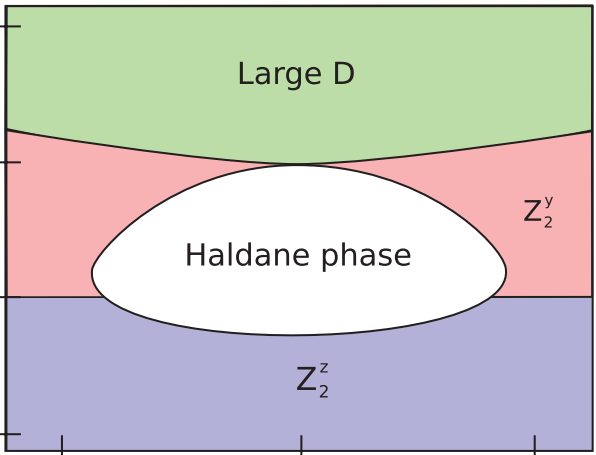
\includegraphics[width=\columnwidth]{diagrams/aklt2.png}
        \end{figure}
    \end{column}
    \begin{column}[T]{.55\textwidth}
    \vskip-0.8cm
    Two distinct featureless insulators:
    \bi 
    \item Large-D phase
    \bi 
    \item Contains product state wavefunction $\ket{\psi} = \ket{000...}$ 
    \ei
    \item Haldane phase
    \bi 
    \item Contains AKLT wavefunction $\ket{\psi} = \Sigma\ket{+00-0+...}$
    \ei 
        \begin{figure}[h]
            \hspace{-2cm}
            \scalebox{1.2}{
            \begin{frame}{MPS Example: AKLT State}
\vskip-1.5cm
\begin{block}{Haldane Phase for Spin-1 chains $(j=1, m=0)$}
\vskip-0.8cm
$$
H_{AKLT} = \sum\limits_{i} J \vec{S}_i\cdot \vec{S}_{i+1} + J' (\vec{S}_i\cdot \vec{S}_{i+1})^2 + D (S^z_i)^2+BS^x
$$
\end{block}
\begin{columns}[T]
    \begin{column}[T]{.45\textwidth}
        \vskip-1.2cm
        \begin{figure}
        \centering
        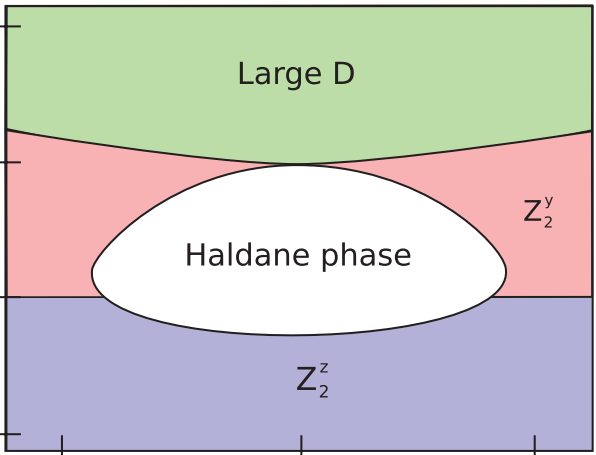
\includegraphics[width=\columnwidth]{diagrams/aklt2.png}
        \end{figure}
    \end{column}
    \begin{column}[T]{.55\textwidth}
    \vskip-0.8cm
    Two distinct featureless insulators:
    \bi 
    \item Large-D phase
    \bi 
    \item Contains product state wavefunction $\ket{\psi} = \ket{000...}$ 
    \ei
    \item Haldane phase
    \bi 
    \item Contains AKLT wavefunction $\ket{\psi} = \Sigma\ket{+00-0+...}$
    \ei 
        \begin{figure}[h]
            \hspace{-2cm}
            \scalebox{1.2}{
            \input{diagrams/aklt.tex}
            }
        \end{figure}

    \ei
    \end{column}
\end{columns}

\end{frame}
            }
        \end{figure}

    \ei
    \end{column}
\end{columns}

\end{frame}
            }
\end{figure}
\begin{columns}[T]
\begin{column}[T]{.5\textwidth}
\vskip-1.5cm
\begin{figure}
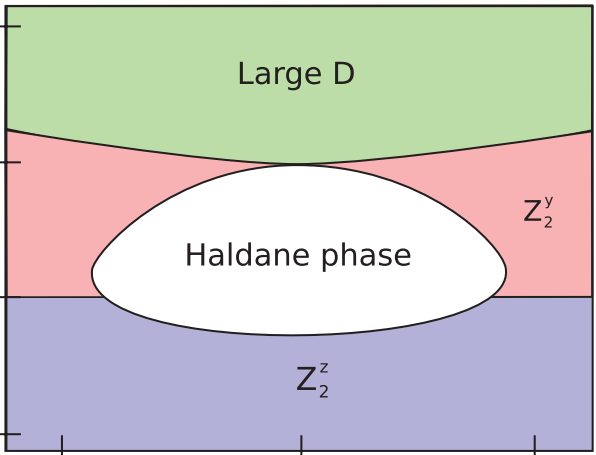
\includegraphics[width=\columnwidth]{diagrams/aklt2.png}
\end{figure}
\end{column}
   \begin{column}[T]{.5\textwidth}
   \vskip-1cm
    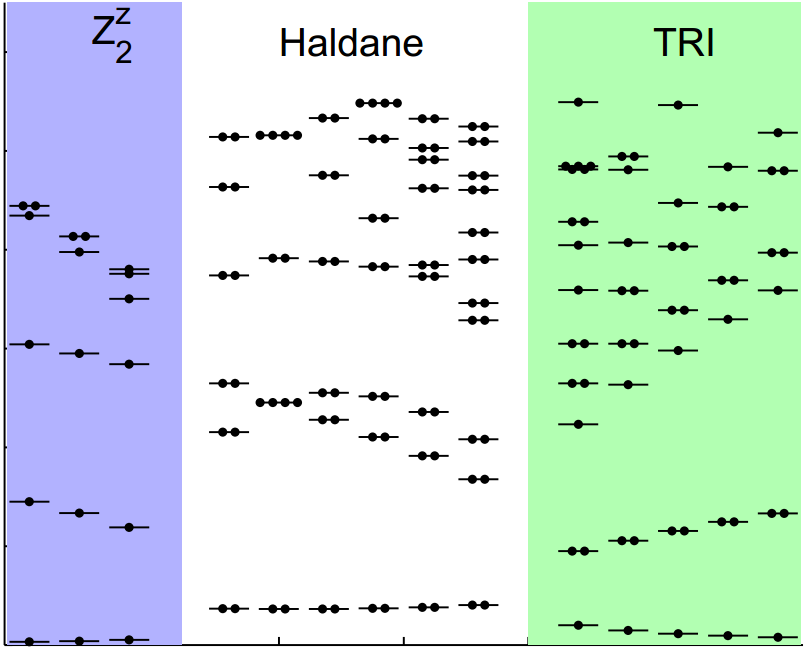
\includegraphics[width=\columnwidth]{diagrams/akltEE.png}
    \end{column}
\end{columns}

Haldane phase distinguished by exact double degeneracy in entire  entanglement spectrum.
\end{frame}
\begin{frame}{2D SPT Example: Chern Insulator}
\vskip-1.5cm
\begin{columns}[T]
\begin{column}[T]{.7\textwidth}
\begin{figure}
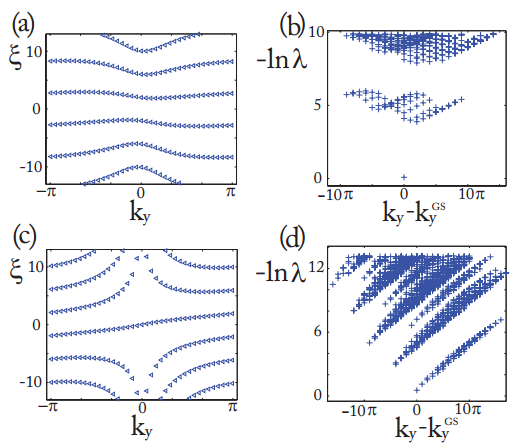
\includegraphics[width=\columnwidth]{diagrams/freefermionEE.png}
\end{figure}
\end{column}
\begin{column}[T]{.3\textwidth}
\bi 
\item Start with 'single particle entanglement spectra' of restricted correlation matrix $C_{ij}$
\item Transform the eigenvalues using $\log{\frac{C}{1-C}}$
\item Fill up to 'zero'
\item Result: Entanglement spectra
\ei
\end{column} 
\end{columns}

\end{frame}

\section{Tensor Networks}
\begin{frame}{What is a matrix product state?}
\vskip-1.5cm
Matrix product states provide a parameterization of the space of wavefunctions of a 1D or quasi-1D system.
\only<1, 3->{
\begin{figure}[h]
    \centering
    \scalebox{1}{
    \begin{tikzpicture}[node distance=0.4cm]
\tikzset{gamma/.style={circle=2pt,draw=black!100, very thick, fill=blue!40, inner sep=3pt}}


\begin{scope}[decoration={
    markings,
    mark=at position 0.5 with {\arrow{>}}}
    ]

\foreach \i in {1,...,6} {
	\node[gamma] (G\i) at (1.5*\i,0) {$A$};
	\node (l\i) at ($ (G\i) + (0, 1) $) {$$};
	\draw[very thick, red!100, postaction={decorate}] (G\i) -- (l\i);
	%\node[below of=G\i] {$A$};
}

\foreach \i in {7} {
	\node[] (G\i) at (1.5*\i,0) {$...$};
    }  
    
\foreach \i / \j in {1/2,2/3,3/4,4/5,5/6, 6/7} {
	\draw[very thick, postaction={decorate}] (G\j) -- (G\i);
}
\node (b0) at (0, 0) {$...$};
\draw[very thick, postaction={decorate}] (G1) -- (b0);

\end{scope}
\end{tikzpicture}

    }
\end{figure}
\only<1>{
$$
\ket{\psi^{b_0 b_1}} = \sum\limits_{p_1 ... p_5}   \vbra{b_0} A^{p_1}_1 ... A^{p_5}_5 \vket{b_1}\ket{p_1 ... p_5} 
$$
}
Coefficients of the wavefunction are calculated via a product of matrices, one per site. The matrix at each site depends on the physical state at that site.
}

\only<2>{
\begin{figure}[h]
    \centering
    \scalebox{1}{
    \begin{tikzpicture}[node distance=0.4cm]
\begin{scope}[decoration={
    markings,
    mark=at position 0.5 with {\arrow{>}}}
    ]
\foreach \i in {1,...,5} {
	\node[gamma] (G\i) at (1.5*\i,0) {};
	\node (l\i) at ($ (G\i) + (0, 1) $) {$p_\i$};
	\draw[thick] (G\i) -- (l\i);
	\node[below of=G\i] {$A^\i$};
}
\foreach \i / \j in {1/2,2/3,3/4,4/5} {
	\draw[thick, postaction={decorate}] (G\j) -- (G\i);
}
\node[side] (B) at (0.5, 0) {$B$};
%\node (b1) at (0, 0) {$b_1$};
\draw[thick, postaction={decorate}] (G1) -- node[below]{$b_0$}(B);
\draw[thick, postaction={decorate}] (8.1, 0)--(G5.east);
\draw[thick, postaction={decorate}] (B.west) -- node[below]{$b_1$}(-0.1, 0);
\end{scope}
\draw[thick, dashed] (0.2,0) .. controls (-1,0) and (-0.6,0.6) .. (4,0.5) .. controls (8.5,0.5) and (9,0) .. (7.5,0);
\end{tikzpicture}
    }
\end{figure}

\only<2>{
$$
\ket{\psi} = \sum\limits_{p_1 ... p_5}   Tr(B A^{p_1}_1 ... A^{p_5}_5)\ket{p_1 ... p_5} 
$$
}

}
\only<3->{
Every state has a matrix product state representation formed through the process of repeated SVD.

\only<3>{
\begin{figure}[h]
    \centering
    \scalebox{1.1}{
    \begin{tikzpicture}[node distance=0.6cm]

\node[side, minimum width=1.6cm, minimum height=0.8cm] (psi) at (0,0) {$\psi$};
\node[above=of psi.north west, anchor=south west] (p1) {};
\node[above=of psi](p2) {};
\node[above=of psi.north east, anchor=south east] (p3) {};
\node at (1.3, 0) {=}; 
\node[cside] (psi1) at (2.2,0) {$U_1$};
\node[lambda] (S) at (3.4, 0) {};
\node[cside] (psiR) at (4.8,0) {$V_1$};
\node[above=of psi1.north west, anchor=south west] (pL) {};
\node[above=of psiR.north west, anchor=south west] (q2) {};
\node[above=of psiR.north east, anchor=south east] (qR) {};

\begin{scope}[decoration={
    markings,
    mark=at position 0.5 with {\arrow{>}}}
    ]
 \draw[->] (psi.north -| p1) -- node[left] {$p_1$} (p1);
 \draw[->] (psi) --  node[left] {$p_2$} (p2);
 \draw[->] (psi.north -| p3) -- node[left] {$p_3$} (p3);
 \draw[->] (psi1.north -| pL) -- node[left] {$p_1$} (pL);
 \draw[->] (psiR.north-|q2)-- node[left] {$p_2$} (q2);
 \draw[->] (psiR.north -| qR) -- node[right] {$p_3$} (qR);
 \draw[-, thick, postaction={decorate}]  (S) -- (psi1);
 \draw[-, thick, postaction={decorate}] (S) -- (psiR);
 \end{scope}
 \end{tikzpicture}
    }
    \note{Maximum bond dimension d}
\end{figure}
}
\only<4>{
\begin{figure}[h]
    \centering
    \scalebox{1.1}{
    \begin{tikzpicture}[node distance=0.6cm]
    \node[side, minimum width=1.5cm, minimum height=0.8cm] (psi) at (0,0) {$\psi$};
    \node[above=of psi.north west, anchor=south west] (p1) {};
    \node[above=of psi](p2) {};
    \node[above=of psi.north east, anchor=south east] (p3) {};
    \node at (1.3, 0) {=}; 
    \node[cside] (psi1) at (2,0) {$U_1$};
    %\node[lambda] (S) at (3, 0) {};
    \node[side,minimum width=1cm, minimum height=0.8cm] (psiR) at (4.2,0) {$\psi'$};
    \node[above=of psi1.north west, anchor=south west] (pL) {};
    \node[above=of psiR.north west, anchor=south west] (q2) {};
    \node[above=of psiR.north east, anchor=south east] (qR) {};
\begin{scope}[decoration={
    markings,
    mark=at position 0.5 with {\arrow{>}}}
    ]
    \draw[->] (psi.north -| p1) -- node[left] {$p_1$} (p1);
    \draw[->] (psi) --  node[left] {$p_2$} (p2);
    \draw[->] (psi.north -| p3) -- node[left] {$p_3$} (p3);
    \draw[->] (psi1.north -| pL) -- node[left] {$p_1$} (pL);
    \draw[->] (psiR.north-|q2)-- node[left] {$p_2$} (q2);
    \draw[->] (psiR.north -| qR) -- node[right] {$p_3$} (qR);
    \draw[-, thick, postaction={decorate}] (psiR) -- node[above]{$i_1$}(psi1);
  \end{scope}
\end{tikzpicture}
    }
    \note{Maximum bond dimension d^2}
\end{figure}
}
\only<5>{
\begin{figure}[h]
    \centering
    \scalebox{1.1}{
    \begin{tikzpicture}[node distance=0.6cm]
    \node[side, minimum width=1.5cm, minimum height=0.8cm] (psi) at (0,0) {$\psi$};
    \node[above=of psi.north west, anchor=south west] (p1) {};
    \node[above=of psi](p2) {};
    \node[above=of psi.north east, anchor=south east] (p3) {};
    \node at (1.3, 0) {=};
    \node[cside] (B1) at (2,0) {$U_1$};
    \node[cside] (B2) at (3.5,0) {$U_2$};
    \node[side, minimum width=0.5cm, minimum height=0.8cm](psiR) at (5, 0){$\psi''$};
    %\node[lambda] (S) at (3, 0) {};
    %\node[side,minimum width=1cm, minimum height=0.8cm] (psiR) at (4.2,0) {$\psi'$};
    \node[above=of B1.north, anchor=south] (pL) {};
    \node[above=of B2] (q2) {};
    %\node[above=of psiR.north west, anchor=south west] (q2) {};
    \node[above=of psiR.north, anchor=south] (qR) {};
\begin{scope}[decoration={
    markings,
    mark=at position 0.5 with {\arrow{>}}}
    ]
    \draw[->] (psi.north -| p1) -- node[left] {$p_1$} (p1);
    \draw[->] (psi) --  node[left] {$p_2$} (p2);
    \draw[->] (psi.north -| p3) -- node[left] {$p_3$} (p3);
    \draw[->] (B1.north -| pL) -- node[left] {$p_1$} (pL);
    \draw[->] (B2.north-|q2)-- node[left] {$p_2$} (q2);
    \draw[->] (psiR.north -| qR) -- node[right] {$p_3$} (qR);
    \draw[-, thick, postaction={decorate}] (B2) -- node[above]{$i_1$}(B1);
    \draw[-, thick, postaction={decorate}] (psiR) -- node[above]{$i_2$}(B2);
 %\draw[-] (psiR) -- (S);
  \end{scope}
\end{tikzpicture}
    }
\end{figure}
}
}

\end{frame}
\begin{frame}{Tensor Network States}
\vskip-1.5cm
\begin{columns}[T]
\begin{column}[T]{.5\textwidth}
\bi
\item MPS and the generalization to PEPS automatically satisfy area law.

\item Entanglement rank and entropy bounded by total bond dimension across any cut.

\item Can view PEPS on cylinder as a MPS.
\ei 
\end{column}
\begin{column}{.5\textwidth}
\vskip-0.7cm
\begin{figure}
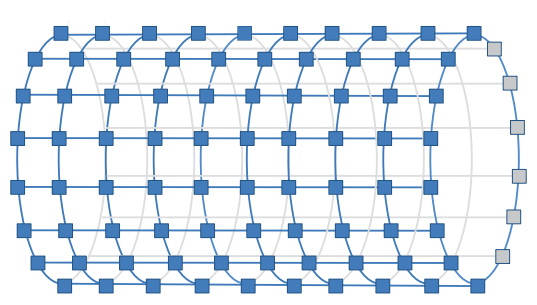
\includegraphics[width=6cm]{diagrams/CylPEPS1.png}
\caption{Translationally symmetric PEPS on a cylinder}
\end{figure}
\vskip-0.6cm
\begin{figure}
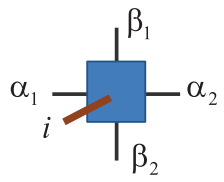
\includegraphics[width=2cm]{diagrams/CylPEPS2.png}
\caption{Close-up of site-tensor in PEPS}
\end{figure}
\end{column}
\end{columns}
\end{frame}
\begin{frame}{Computing Correlation Functions in MPS}
\vskip-1.5cm
\only<1,3->{
\begin{figure}[t]
\centering
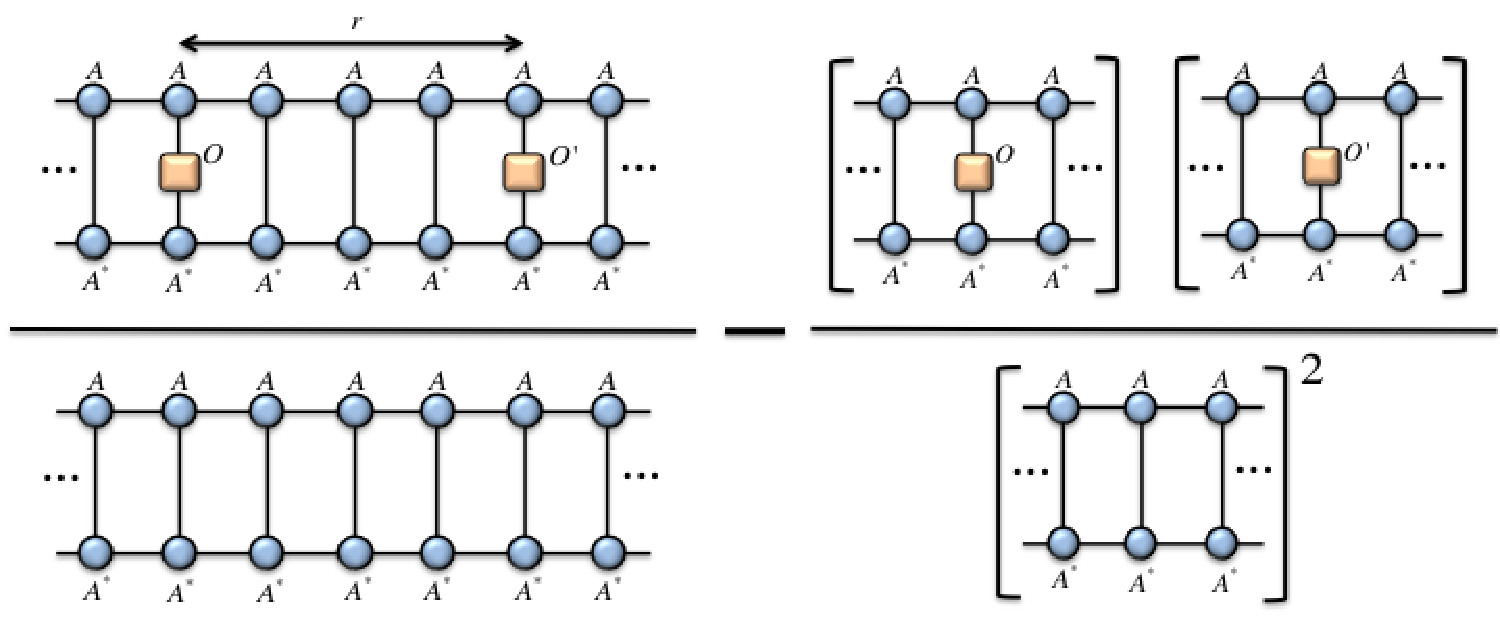
\includegraphics[width=\textwidth]{diagrams/orus-corrfunc.pdf}
%\begin{tikzpicture}[node distance=0.5cm]

\foreach \i in {1,...,5} {
	\node (Gp\i) at (1.5*\i,-2.5) [gamma] {};
	\node (Gpp\i) at ($ (Gp\i) + (0,-1) $) [gamma] {};
	\draw[thick] (Gp\i) -- (Gpp\i);
	\node[above of=Gp\i] {$A^\i$};
	\node[below of=Gpp\i] {$(A^\i)^*$};
}
\foreach \i / \j in {1/2,2/3,3/4,4/5} {
	\draw[thick] (Gp\i) -- (Gp\j);
	\draw[thick] (Gpp\i) -- (Gpp\j);
}

\foreach \i in {1,...,5} {
	\node (Gp\i) at (1.5*\i,-5.5) [gamma] {};
	\node (Gpp\i) at ($ (Gp\i) + (0,-2) $) [gamma] {};
	\node (O\i) at ($ (Gp\i) + (-0,-1) $) [operator] {};
	
	\draw[thick] (Gp\i) -- (O\i);
	\draw[thick] (Gpp\i) -- (O\i);
	
	\node[above of=Gp\i] {$A^\i$};
	\node[below of=Gpp\i] {$(A^\i)^*$};
	\node[above left of=O\i] {$W^\i$};
}
\foreach \i / \j in {1/2,2/3,3/4,4/5} {
	\draw[thick] (Gp\i) -- (Gp\j);
	\draw[thick] (Gpp\i) -- (Gpp\j);
	\draw[thick] (O\i) -- (O\j);
}

\end{tikzpicture}

\caption{Diagram for $C_{O O'}(r) = \ev{O_i O'_{i+r}}- \ev{O_i}\ev{O'_{i+r}}$}
\end{figure}
}
\only<2>{
\begin{columns}[T]
    \begin{column}[T]{.28\textwidth}
        \begin{figure}[h]
            \centering
            \scalebox{1}{
            \begin{tikzpicture}[node distance=0.4cm]
\begin{scope}[thick, decoration={
    markings,
    mark=at position 0.5 with {\arrow{>}}}
    ]
  \node[gamma] (A) at (0,0) {$A$};  
  \node[gamma] (Ac) at (0,2) {$A^{*}$};
  \draw[postaction={decorate}] (A)--(Ac);
  \node[inv] (ki) at (1, 0){};
  \node[inv] (bi) at (1, 2){}; 
  \node[inv] (ko) at (-1, 0){}; 
  \node[inv] (bo) at (-1, 2){};
  \draw[color=red, postaction={decorate}] (ki)--(A);
  \draw[color=green, postaction={decorate}] (bi)--(Ac);
  \draw[color=red, postaction={decorate}] (A) -- (ko);
  \draw[color=green, postaction={decorate}] (Ac) -- (bo);

\end{scope}
\end{tikzpicture}

            }
            \caption{Transfer Matrix $\mathbb{E}_{I}$}
            \note{Reminder using arrows to represent in and out}
        \end{figure}
    \end{column}
    \begin{column}[T]{.3\textwidth}
        \begin{figure}[h]
            \centering
            \scalebox{1}{
            \begin{tikzpicture}[node distance=0.4cm]
\begin{scope}[thick, decoration={
    markings,
    mark=at position 0.5 with {\arrow{>}}}
    ]
  \node[gamma] (A) at (0,0) {$A$};  
  \node[operator] (O) at (0, 1) {$O$};
 % \node[operator] (O2) at (0, 1) {$O'$};
  \node[gamma] (Ac) at (0,2) {$A^{*}$};
  \draw[postaction={decorate}] (A)-- (O) -- (Ac);
  \node[inv] (ki) at (1, 0){};
  \node[inv] (bi) at (1, 2){}; 
  \node[inv] (ko) at (-1, 0){}; 
  \node[inv] (bo) at (-1, 2){};
  \draw[color=red, postaction={decorate}] (ki)--(A);
  \draw[color=green, postaction={decorate}] (bi)--(Ac);
  \draw[color=red, postaction={decorate}] (A) -- (ko);
  \draw[color=green, postaction={decorate}] (Ac) -- (bo);

\end{scope}
\end{tikzpicture}
            }
            \caption{Operator Insertion $\mathbb{E}_{O}$}
        \end{figure}
    \end{column}
    \begin{column}[T]{.42\textwidth}
        \vskip1.8cm
        \begin{figure}[h]
            \centering
            \scalebox{0.8}{
            \begin{tikzpicture}
\begin{scope}[very thick,decoration={
    markings,
    mark=at position 0.5 with {\arrow{>}}}
    ] 

\node[peps] (A1) at (-4.1, 0) {};
\node (li) at ($(A1) + (-1, 0) $) {};
\draw[thick, postaction={decorate}] (li.center) -- (A1.west);
\draw[thick, postaction={decorate}] (A1.east) -- node[right] {} +(1,0);
\draw[thick, postaction={decorate}] (A1.north) -- node[above] {} +(0,0.5);

\node at (-2.3, 0.5){$= e^{i \theta}$};    

\node[peps] (A) at (0, 0) {};
\node[draw] (Ul) at ($(A) + (-1, 0) $) {$U$};
\node[draw] (Ur) at ($(A) + (1, 0) $) {$U^{\dagger}$};
\node (LI) at ($(Ul) + (-1, 0) $) {};
\draw[thick, postaction={decorate}] (LI.center) -- (Ul.west);
\draw[thick, postaction={decorate}] (Ur.east) -- node[right] {} +(0.5,0);
\draw[thick, postaction={decorate}] (Ul) -- (A);
\draw[thick, postaction={decorate}] (A) -- (Ur);
\draw[thick, postaction={decorate}] (A.north) -- node[above] {} +(0,0.5);

\end{scope}
\end{tikzpicture}
            }
            \caption{MPS gauge redundancy}
        \end{figure}
    \end{column}
\end{columns} 
\begin{figure}[h]
    \centering
    \scalebox{1}{
    \begin{tikzpicture}[node distance=0.4cm]
\begin{scope}[thick, decoration={
    markings,
    mark=at position 0.5 with {\arrow{>}}}
    ]
  \node[gamma] (A) at (0,0) {$A$};  
  \node[gamma] (Ac) at (0,2) {$A^{*}$};
  \node[side, minimum height=1.97cm] (vR) at (1.5, 1){$v_R$};
  \draw[postaction={decorate}] (A)--(Ac);
  \node[inv] (ki) at (1, 0){};
  \node[inv] (bi) at (1, 2){}; 
  \node[inv] (ko) at (-1, 0){}; 
  \node[inv] (bo) at (-1, 2){};
  \draw[color=red, postaction={decorate}] (vR.south west) -- (ki.center)--(A);
  \draw[color=green, postaction={decorate}] (vR.north west)-- (bi.center)--(Ac);
  \draw[color=red, postaction={decorate}] (A) -- (ko);
  \draw[color=green, postaction={decorate}] (Ac) -- (bo);
  
  \node[] at (2.5, 1){$=$};
  \node[side, minimum height=1.97cm] (vR) at (3.5, 1){$v_R$};
  \node[inv] (ki) at (2.5, 0){};
  \node[inv] (bi) at (2.5, 2){};
  \draw[color=red, postaction={decorate}] (vR.south west) -- (ki.center);
  \draw[color=green, postaction={decorate}] (vR.north west)-- (bi.center); 

  \node[] at (4.5, 1){$=$};
  \node[side, minimum height=0.6cm] (sR) at (5.5, 0){$\sigma_R$};
  \node[inv] (ki) at (4.5, 0){};
  \node[inv] (k2) at (6.3, 0){};
  \node[cdot] (dot) at (6.3, 1){};
   \node[inv] (b2) at (6.3, 2){};
  \node[inv] (bi) at (4.5, 2){};
  \draw[color=red, postaction={decorate}]  (dot)--(k2.center);
  \draw[color=red, postaction={decorate}]  (k2.center)-- (sR.east);
  \draw[color=red, postaction={decorate}]  (sR.west) -- (ki.center);
  \draw[color=green, postaction={decorate}]  (dot)--(b2.center);
  \draw[color=green, postaction={decorate}]  (b2.center)-- (bi);
\end{scope}
\end{tikzpicture}
    }
\caption{Eigenvector equation $\mathbb{E}_{I}(\sigma_R) = \sigma_R$}
\end{figure}
   
}
\only<3>{
\vskip-0.5cm
 $$\ev{O_i O'_{i+r}} = \vbraopket{v_L}{\mathbb{E}_O \mathbb{E}_I^r \mathbb{E}_{O'}}{v_R}$$
 $$
 \lim\limits_{r \rightarrow \infty} \ev{O_i O'_{i+r}} = \vbraopket{v_L}{\mathbb{E}_O}{v_R} \vbraopket{v_L}{\mathbb{E}_{O'}}{v_R}
 $$
 $$ C_{O O'}(r) \approx const. \times \lambda_2^r $$
\note{Matrix product states also known as finitely correlated states}
}
\end{frame}

\begin{frame}{Computing Entanglement in MPS/PEPS}
\vskip-1.5cm
To compute the spectrum of the reduced density matrix 
\only<1, 2>{
\begin{figure}
\scalebox{1}{
            \begin{tikzpicture}[node distance=0.4cm]
\begin{scope}[decoration={
    markings,
    mark=at position 0.5 with {\arrow{>}}}
    ]
\node[] (rho) at (-0.5,1) {\Large $\rho =$};      
\foreach \i in {1,...,3} {
	\node[gamma] (G\i) at (1.5*\i,0) {$A$};
	\node (l\i) at ($ (G\i) + (0, 1) $) {$$};
	\draw[thick, postaction={decorate}] (G\i) -- (l\i);
	%\node[below of=G\i] {$A$};
}
\foreach \i / \j in {1/2,2/3} {
	\draw[thick, postaction={decorate}] (G\j) -- (G\i);
}
\node (b0) at (0, 0) {$...$};
\draw[thick, postaction={decorate}] (G1) -- (b0);

\foreach \i in {1,...,3} {
	\node[gamma] (B\i) at (1.5*\i,2) {$A^*$};
	\node (l\i) at ($ (B\i) + (0, -1) $) {$$};
	\draw[thick, postaction={decorate}] (l\i) -- (B\i);
	%\node[below of=G\i] {$A$};
}
\foreach \i / \j in {1/2,2/3} {
	\draw[thick, postaction={decorate}] (B\i) -- (B\j);
}
\node (b1) at (0, 2) {$...$};
\draw[thick, postaction={decorate}] (b1) -- (B1);

\foreach \i in {4,...,6} {
	\node[gamma] (G\i) at (1.5*\i,0) {$A$};
	\node[gamma] (B\i) at (1.5*\i,2) {$A^*$};
	\draw[thick, postaction={decorate}] (G\i) -- (B\i);
	}
\foreach \i in {7} {
	\node[] (G\i) at (1.5*\i,0) {$...$};
	\node[] (B\i) at (1.5*\i,2) {$...$};
    }  
\foreach \i / \j in {3/4,4/5,5/6, 6/7} {
	\draw[thick, postaction={decorate}] (G\j) -- (G\i);
	\draw[thick, postaction={decorate}] (B\i) -- (B\j);
}
\end{scope}
\end{tikzpicture}

            }
\end{figure}
}

\only<3>{
\begin{figure}
\scalebox{1}{
            \begin{tikzpicture}[node distance=0.4cm]
\begin{scope}[decoration={
    markings,
    mark=at position 0.5 with {\arrow{>}}}
    ]
\node[] (rho) at (4.5,1) {\Large $\widetilde{\rho} =$};  

\foreach \i in {3} {
	\node[inv] (G\i) at (1.5*\i,0) {$A$};
	\node[inv] (B\i) at (1.5*\i,2) {$A^*$};
    }
\foreach \i in {7} {
	\node[] (G\i) at (1.5*\i,0) {$...$};
	\node[] (B\i) at (1.5*\i,2) {$...$};
    }    
\foreach \i in {4,...,6} {
	\node[gamma] (G\i) at (1.5*\i,0) {$A$};
	\node[gamma] (B\i) at (1.5*\i,2) {$A^*$};
	\draw[thick, postaction={decorate}] (G\i) -- (B\i);
	}
\foreach \i / \j in {3/4,4/5,5/6, 6/7} {
	\draw[thick, postaction={decorate}] (G\j) -- (G\i);
	\draw[thick, postaction={decorate}] (B\i) -- (B\j);
}
\end{scope}
\end{tikzpicture}

            }
\end{figure}
}
\only<2>{
A valid simplified case is when the contraction 
\begin{figure}
\scalebox{1}{
            \begin{tikzpicture}[node distance=0.4cm]
\begin{scope}[decoration={
    markings,
    mark=at position 0.5 with {\arrow{>}}}
    ]
\node[] (u) at (-0.5, 0) {\Large $\mathcal{U} =$}; 
\foreach \i in {1,...,3} {
	\node[gamma] (G\i) at (1.5*\i,0) {$A$};
	\node (l\i) at ($ (G\i) + (0, 1) $) {$$};
	\draw[thick, postaction={decorate}] (G\i) -- (l\i);
	%\node[below of=G\i] {$A$};
}
\foreach \i / \j in {1/2,2/3} {
	\draw[thick, postaction={decorate}] (G\j) -- (G\i);
}
\node (b0) at (0, 0) {$...$};
\node[inv] (sigL) at (6, 0) {$\frac{1}{\sqrt{\sigma_L}}$};
\draw[thick, postaction={decorate}] (G1) -- (b0);
\draw[thick, postaction={decorate}] (sigL) -- (G3);
%\node[inv](Q) at (7, 0){};
%\draw[thick, postaction={decorate}] (Q) -- (sigL);
\end{scope}
\end{tikzpicture}

            }
\end{figure}

is isometric. We can always get into this canonical form.
}


\only<3>{
\bi 
\item $\rho = \mathcal{U} \cdot \widetilde{\rho} \cdot \mathcal{U}^{\dagger}$
\item $\widetilde{\rho}$ is isometric to real $\rho$ - same spectrum, many less 0s.
\ei
}
\end{frame}
\begin{frame}{PEPS Construction of Honeycomb F.B.I.}
\vskip-1.5cm
A wavefunction written as a product of local operators acting on a product state can be turned into a tensor network.

\only<1>{
\begin{figure}[h]
\scalebox{1}{
% y=\sqrt{3/4}*(minimum size)/2
%

%http://tex.stackexchange.com/questions/6019/drawing-hexagons
\begin{tikzpicture}[x=7.5mm,y=4.33mm]
  % some styles
  \tikzset{
    box/.style={
      regular polygon,
      regular polygon sides=6,
      minimum size=10mm,
      inner sep=0mm,
      outer sep=0mm,
      rotate=0,
     dotted,
     thin,
      black,
      draw
    }
  }
  \tikzset{
    bbox/.style={
      regular polygon,
      regular polygon sides=6,
      minimum size=7mm,
      %fill,
      inner sep=0mm,
      outer sep=0mm,
      rotate=0,
     % dotted,
     very thick,
     orange,
      draw
    }
  }
    \tikzset{
    wb/.style={
       regular polygon,
      regular polygon sides=6,
      minimum size=5mm,
      %fill,
      inner sep=0mm,
      outer sep=0mm,
      rotate=0,
     % dotted,
     very thick,
     green,
      draw
    }
  }
 \tikzset{boson/.style={circle=1pt,draw=black!100,fill=orange!100,inner sep=2pt}}
  \tikzset{dimer/.style={ellipse=1pt,draw=black!100,fill=orange!90,inner sep=2pt}}
    \tikzset{thindimer/.style={ellipse=1pt,draw=black!100,fill=orange!90,inner sep=1pt}}
\tikzset{peps/.style={circle=2pt,draw=black!100,fill=green!50,inner sep=3pt}}
\tikzset{bpeps/.style={circle=2pt,draw=black!100,thick,fill=green!50,inner sep=3pt}}
\tikzset{gamma/.style={circle=2pt,draw=black!100,fill=blue!50,inner sep=3pt}}
\tikzset{lambda/.style={rectangle,rotate=45,draw=black!100,fill=red!50,inner sep=2pt}}
\tikzset{operator/.style={circle=1pt,draw=black!100,fill=blue,inner sep=1.5pt}}

\foreach \i in {0,...,2} 
    \foreach \j in {0,...,2} {
    \pgfmathtruncatemacro{\x}{2*\i}
    \pgfmathtruncatemacro{\y}{2*\j}
            \node[box] (H\x\y) at (\x,\y) {};
             \node[wb] (W\x\y) at (\x,\y) {};
              \node[green] at (\x, \y) {\tiny W};
             \foreach \k in {1, ..., 6}{
             \node[operator] (D\x\y\k) at (H\x\y.corner \k) {};
             \draw[ blue] (W\x\y) -- (D\x\y\k);
             }
        }
\foreach \i in {0,1} 
    \foreach \j in {0,..., 2} {
        \pgfmathtruncatemacro{\x}{2*\i+1}
    \pgfmathtruncatemacro{\y}{2*\j+1}
   	  \node[box] (H\x\y) at (\x,\y) {};   
   	   \node[wb] (W\x\y) at (\x,\y) {};
   	    \node[green] at (\x, \y) {\tiny W};
             \foreach \k in {1, ..., 6}{
             \node[operator] (D\x\y\k) at (H\x\y.corner \k) {};
             \draw[thick, blue] (W\x\y) -- (D\x\y\k);
             }
        }


            %\foreach \k in {1,...,6}{
          %  \node[circle, label=above:\i, fill=red] at (H\i\j.corner \k) {};
           % }
%\node[circle, draw] at (H00.corner 1) {};
\end{tikzpicture}
}
\end{figure}

Virtual W-state on each plaquette used to synchronize the creation operators in the sum $\sum\limits_{i \in \varhexagon} b^{\dagger}_i$
$$\vket{W} = \vket{000001}+\vket{000010}+\vket{000100}+\vket{001000}+\vket{010000}+\vket{100000}$$

}

\only<2>{
\begin{columns}[T]
\begin{column}{0.5\textwidth}
\begin{figure}[h]
\scalebox{1.3}{
\begin{tikzpicture}[x=7.5mm,y=4.33mm]
\begin{scope}[decoration={
    markings,
    mark=at position 0.5 with {\arrow{>}}}
    ]
    
  \tikzset{
    box/.style={
      regular polygon,
      regular polygon sides=6,
      minimum size=15mm,
      inner sep=0mm,
      outer sep=0mm,
      rotate=0,
     dotted,
     thin,
      black,
      draw
    }
    }
      \tikzset{
    abox/.style={
      regular polygon,
      regular polygon sides=6,
      minimum size=9mm,
      inner sep=0mm,
      outer sep=0mm,
      rotate=0,
     dotted,
     thin,
      black,
      draw
    }
    }


    \tikzset{
    wb/.style={
       regular polygon,
      regular polygon sides=6,
      minimum size=4.5mm,
      %fill,
      inner sep=0mm,
      outer sep=0mm,
      rotate=0,
     % dotted,
     very thick,
     blue,
      draw
    }
  }
\tikzset{smalldot/.style={circle=1pt,draw=black!100,fill=black!100,inner sep=1pt}}
\tikzset{smallwdot/.style={circle=1pt, very thick, draw=blue!100,fill=white,inner sep=1pt}}

 \node[box] (H) at (0, 0) {};
\node[wb] (W) at (0,0) {};

\foreach \k in {1, ..., 6}{
             \node[inv] (D\k) at (H.corner \k) {};
             \draw[very thick, black] (W) -- (D\k);
             }
             
 \node[] at (1.5, 0){$=$};

 \node[box] (H3) at (3, 0) {};
 \node[abox] (H2) at (3, 0) {};
%\node[wb] (W) at (3,0) {\tiny W};
\foreach \k in {1, ..., 6}{
             \node[smalldot] (A\k) at (H2.corner \k) {};
             }

\foreach \k in {1,2,3,5}{
		\pgfmathtruncatemacro{\j}{\k+1}
            \draw[thick, postaction={decorate}] (A\k) -- (A\j);
             }
             \draw[thick, postaction={decorate}] (A6) -- (A1);
             
 \foreach \k in {1,2,3,4,5,6}{
            \draw[thick, postaction={decorate}] (A\k) -- (H3.corner \k);
             }
             
 \node[smallwdot](B) at (3, 0) {\tiny 1};
 \draw[thick, postaction={decorate}]  (B)--(A5);

\end{scope}
\end{tikzpicture}
}
\end{figure}
$$\vket{W} = \vket{100...}+...$$
\vskip-0.5cm
\bi 
\item W-State can be factored and put on hexagon sites
\item Each black directed string has either charge $0$ or $1$
\item Charge conserved
\ei 
\end{column}
\begin{column}{0.5\textwidth}
\begin{figure}[h]
\scalebox{1.5}{
\begin{tikzpicture}[x=7.5mm,y=4.33mm]
\begin{scope}[decoration={
    markings,
    mark=at position 0.5 with {\arrow{>}}}
    ]
    
  \tikzset{
    box/.style={
      regular polygon,
      regular polygon sides=6,
      minimum size=15mm,
      inner sep=0mm,
      outer sep=0mm,
      rotate=0,
     dotted,
     thin,
      black,
      draw
    }
    }
      \tikzset{
    abox/.style={
      regular polygon,
      regular polygon sides=6,
      minimum size=9mm,
      inner sep=0mm,
      outer sep=0mm,
      rotate=0,
     dotted,
     thin,
      black,
      draw
    }
    }

  \tikzset{
    bbox/.style={
      regular polygon,
      regular polygon sides=6,
      minimum size=7mm,
      %fill,
      inner sep=0mm,
      outer sep=0mm,
      rotate=0,
     % dotted,
     very thick,
     orange,
      draw
    }
  }
    \tikzset{
    wb/.style={
       regular polygon,
      regular polygon sides=6,
      minimum size=5mm,
      %fill,
      inner sep=0mm,
      outer sep=0mm,
      rotate=0,
     % dotted,
     very thick,
     green,
      draw
    }
  }
 \tikzset{boson/.style={circle=1pt,draw=black!100,fill=orange!100,inner sep=2pt}}
  \tikzset{dimer/.style={ellipse=1pt,draw=black!100,fill=orange!90,inner sep=2pt}}
    \tikzset{thindimer/.style={ellipse=1pt,draw=black!100,fill=orange!90,inner sep=1pt}}
\tikzset{peps/.style={circle=2pt,draw=black!100,fill=green!50,inner sep=3pt}}
\tikzset{bpeps/.style={circle=2pt,draw=black!100,thick,fill=green!50,inner sep=3pt}}
 \tikzset{smalldot/.style={circle=1pt,draw=black!100,fill=black!100,inner sep=1pt}}
  \tikzset{smallwdot/.style={circle=1pt,draw=black!100,fill=orange!50,inner sep=1pt}}
\tikzset{gamma/.style={circle=2pt,draw=black!100,fill=blue!50,inner sep=3pt}}
\tikzset{lambda/.style={rectangle,rotate=45,draw=black!100,fill=red!50,inner sep=2pt}}
\tikzset{operator/.style={circle=1pt,draw=black!100,fill=blue,inner sep=1.5pt}}

 %\node[box] (H) at (0, 0) {};
  %\node[box] (H2) at (1.5, 1.5) {};
   %\node[box] (H3) at (1.5, -1.5) {};
   
   \node[operator] (A) at (1, 0){};
    \draw[thick, postaction={decorate}] (0.5, 0) --node[below]{$i$} (A);
    \draw[thick, postaction={decorate}] (1.25, .75) -- node[right]{$j$}(A);
    \draw[thick, postaction={decorate}] (1.25, -.75) -- node[right]{$k$} (A);
    \draw[red, very thick, postaction={decorate}]  (A)-- node[left]{$p$}(1, 2);


% \foreach \k in {1, ..., 6}{
%              \node[inv] (D\k) at (H.corner \k) {};
%              \draw[ blue] (W) -- (D\k);
%              }
%              
%  \node[] at (1.5, 0){$=$};
%  
%   \node[box] (H) at (0, 0) {};
% \node[wb] (W) at (0,0) {\tiny W};
% 
%  \node[box] (H3) at (3, 0) {};
%  \node[abox] (H2) at (3, 0) {};
% %\node[wb] (W) at (3,0) {\tiny W};
% \foreach \k in {1, ..., 6}{
%              \node[smalldot] (A\k) at (H2.corner \k) {};
%              }
% 
% \foreach \k in {1,2,3,5}{
% 		\pgfmathtruncatemacro{\j}{\k+1}
%             \draw[thick, postaction={decorate}] (A\k) -- (A\j);
%              }
%              \draw[thick, postaction={decorate}] (A6) -- (A1);
%              
%  \foreach \k in {1,2,3,4,5,6}{
%             \draw[thick, postaction={decorate}] (A\k) -- (H3.corner \k);
%              }
%              
%  \node[smallwdot](B) at (3.2, 0) {\tiny 1};
%  \draw[thick, postaction={decorate}]  (B)--(A5);
             
%\foreach \q in {1, ... ,5}{
	%	\pgfmathtruncatemacro{\j}{\k+1}
    %        \draw[] (A.corner \j) -- (A.corner \k);
   %       }

\end{scope}
\end{tikzpicture}
}
\end{figure}
\vskip-0.3cm
\bi 
\item `Projects' the three virtual qubits coming into each vertex on to a state in physical Hilbert space
\item Physical state is either $\ket{0}, \ket{1}, \ket{2}, \ket{3}$
\item Charge conserved
\ei 
\end{column}
\end{columns}
}

\end{frame}
\begin{frame}{Correlations in Honeycomb F.B.Is}
\vskip-1.5cm
\only<1>{
\begin{figure}[hbctp]
\begin{center}
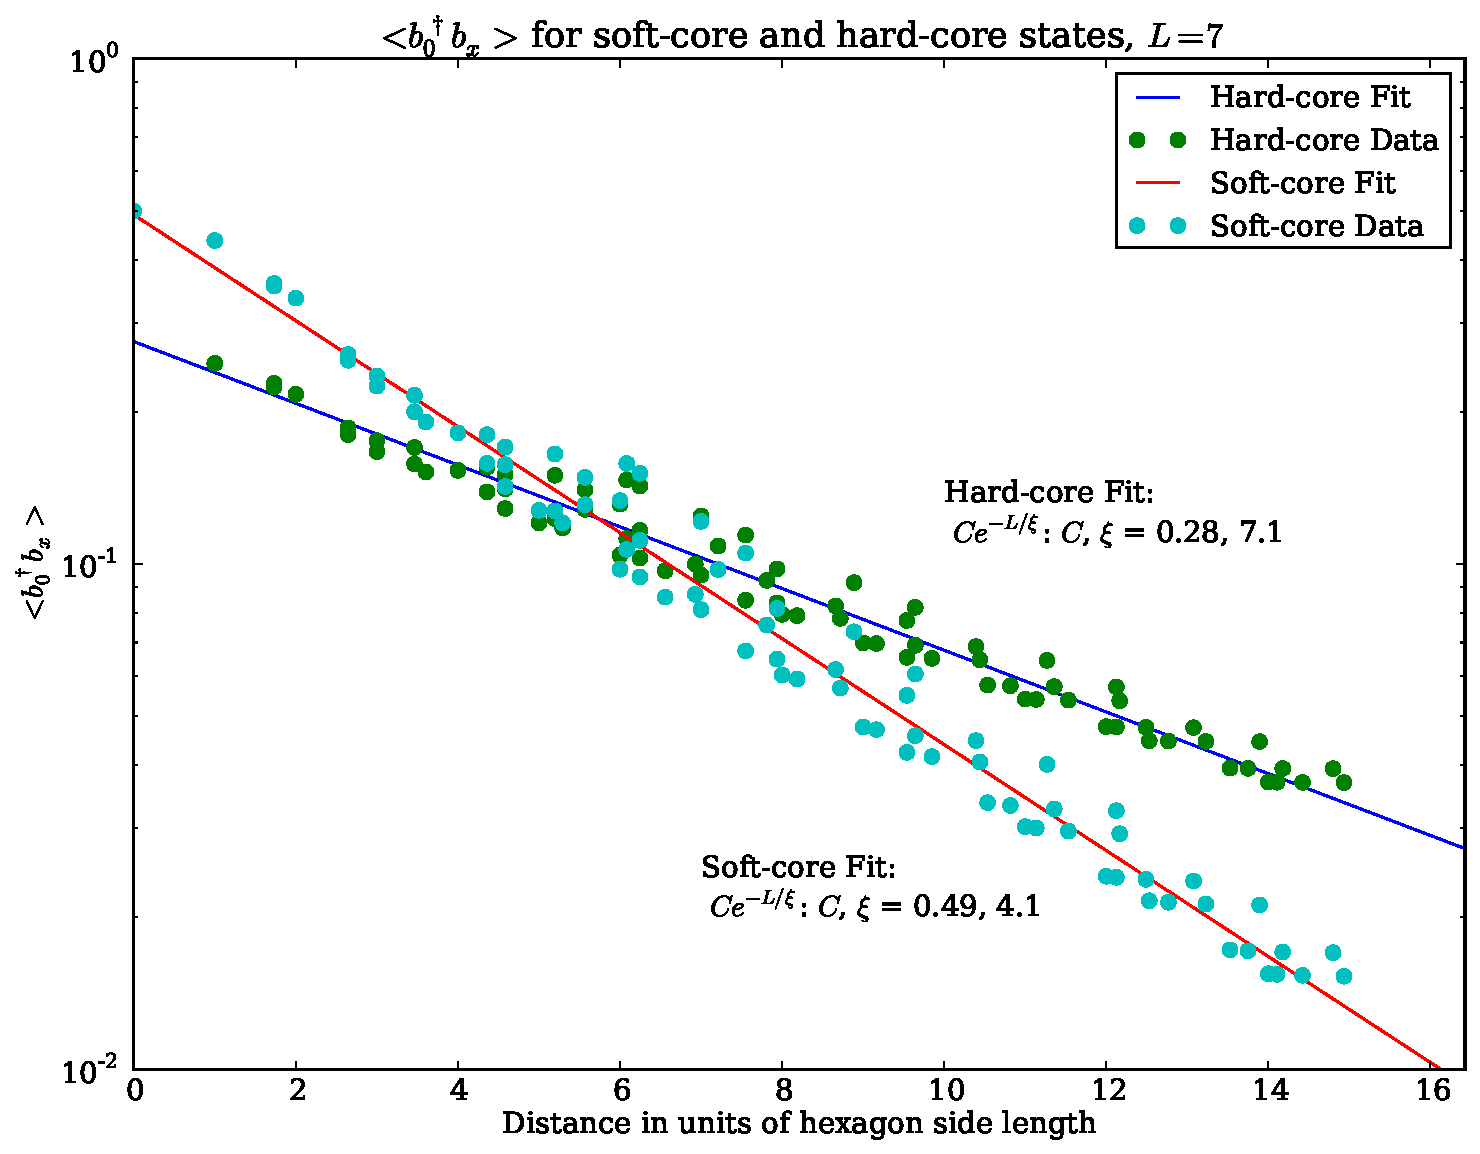
\includegraphics[width=8cm]{{summary/log_bdagb_corr_comparison.pdf}}
\end{center}
\caption{The correlation function $<b_x b^{\dagger}_0>$ shown on a log-scale F.B.I. and hard-core projected version.}
\end{figure}
}
\only<2>{

\begin{figure}[hbctp]
\begin{center}
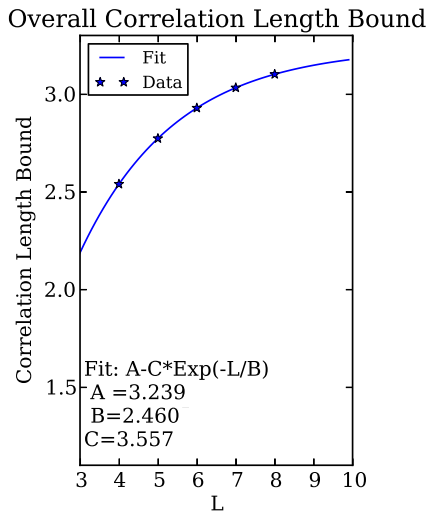
\includegraphics[width=5cm]{diagrams/corrlengthbound.png}
\end{center}
\end{figure}

Evidence for energy gap - exponentially decaying correlations in thermodynamic limit
}
\end{frame}
\section{Entanglement Edge of Honeycomb Insulators}

\begin{frame}{Zig-zag Edge Entanglement Cut}
\vskip-1.5cm
\begin{figure}[h]
\scalebox{1}{
% y=\sqrt{3/4}*(minimum size)/2
%

%http://tex.stackexchange.com/questions/6019/drawing-hexagons
\begin{tikzpicture}[x=7.5mm,y=4.33mm]
  % some styles
  \tikzset{
    box/.style={
      regular polygon,
      regular polygon sides=6,
      minimum size=10mm,
      inner sep=0mm,
      outer sep=0mm,
      rotate=0,
     dotted,
     thin,
      black,
      draw
    }
  }
  \tikzset{
    bbox/.style={
      regular polygon,
      regular polygon sides=6,
      minimum size=7mm,
      %fill,
      inner sep=0mm,
      outer sep=0mm,
      rotate=0,
     % dotted,
     very thick,
     orange,
      draw
    }
  }
    \tikzset{
    wb/.style={
       regular polygon,
      regular polygon sides=6,
      minimum size=5mm,
      %fill,
      inner sep=0mm,
      outer sep=0mm,
      rotate=0,
     % dotted,
     very thick,
     green,
      draw
    }
  }
 \tikzset{boson/.style={circle=1pt,draw=black!100,fill=orange!100,inner sep=2pt}}
  \tikzset{dimer/.style={ellipse=1pt,draw=black!100,fill=orange!90,inner sep=2pt}}
    \tikzset{thindimer/.style={ellipse=1pt,draw=black!100,fill=orange!90,inner sep=1pt}}
\tikzset{peps/.style={circle=2pt,draw=black!100,fill=green!50,inner sep=3pt}}
\tikzset{bpeps/.style={circle=2pt,draw=black!100,thick,fill=green!50,inner sep=3pt}}
\tikzset{gamma/.style={circle=2pt,draw=black!100,fill=blue!50,inner sep=3pt}}
\tikzset{lambda/.style={rectangle,rotate=45,draw=black!100,fill=red!50,inner sep=2pt}}
\tikzset{operator/.style={circle=1pt,draw=black!100,fill=blue,inner sep=1.5pt}}

\foreach \i in {0,...,2} 
    \foreach \j in {0,...,2} {
    \pgfmathtruncatemacro{\x}{2*\i}
    \pgfmathtruncatemacro{\y}{2*\j}
            \node[box] (H\x\y) at (\x,\y) {};
             \node[wb] (W\x\y) at (\x,\y) {};
              \node[green] at (\x, \y) {\tiny W};
             \foreach \k in {1, ..., 6}{
             \node[operator] (D\x\y\k) at (H\x\y.corner \k) {};
             \draw[ blue] (W\x\y) -- (D\x\y\k);
             }
        }
\foreach \i in {0,1} 
    \foreach \j in {0,..., 2} {
        \pgfmathtruncatemacro{\x}{2*\i+1}
    \pgfmathtruncatemacro{\y}{2*\j+1}
   	  \node[box] (H\x\y) at (\x,\y) {};   
   	   \node[wb] (W\x\y) at (\x,\y) {};
   	    \node[green] at (\x, \y) {\tiny W};
             \foreach \k in {1, ..., 6}{
             \node[operator] (D\x\y\k) at (H\x\y.corner \k) {};
             \draw[thick, blue] (W\x\y) -- (D\x\y\k);
             }
        }

\draw[very thick, red] (2, 8) -- (2, -3);
            %\foreach \k in {1,...,6}{
          %  \node[circle, label=above:\i, fill=red] at (H\i\j.corner \k) {};
           % }
%\node[circle, draw] at (H00.corner 1) {};
\end{tikzpicture}
}
\end{figure}
\bi 
\item Cylinder, Circumference $L$
\item Cut crosses $L$ W-strings
\item $\widetilde{\rho} = \exp{-\widetilde{H}}$ is a density matrix on $L$ spin 1/2s 
\ei 
\end{frame}

%\subsection{CFT Identification}
\begin{frame}{Entanglement Spectra}
\vskip-1.5cm
\begin{figure}
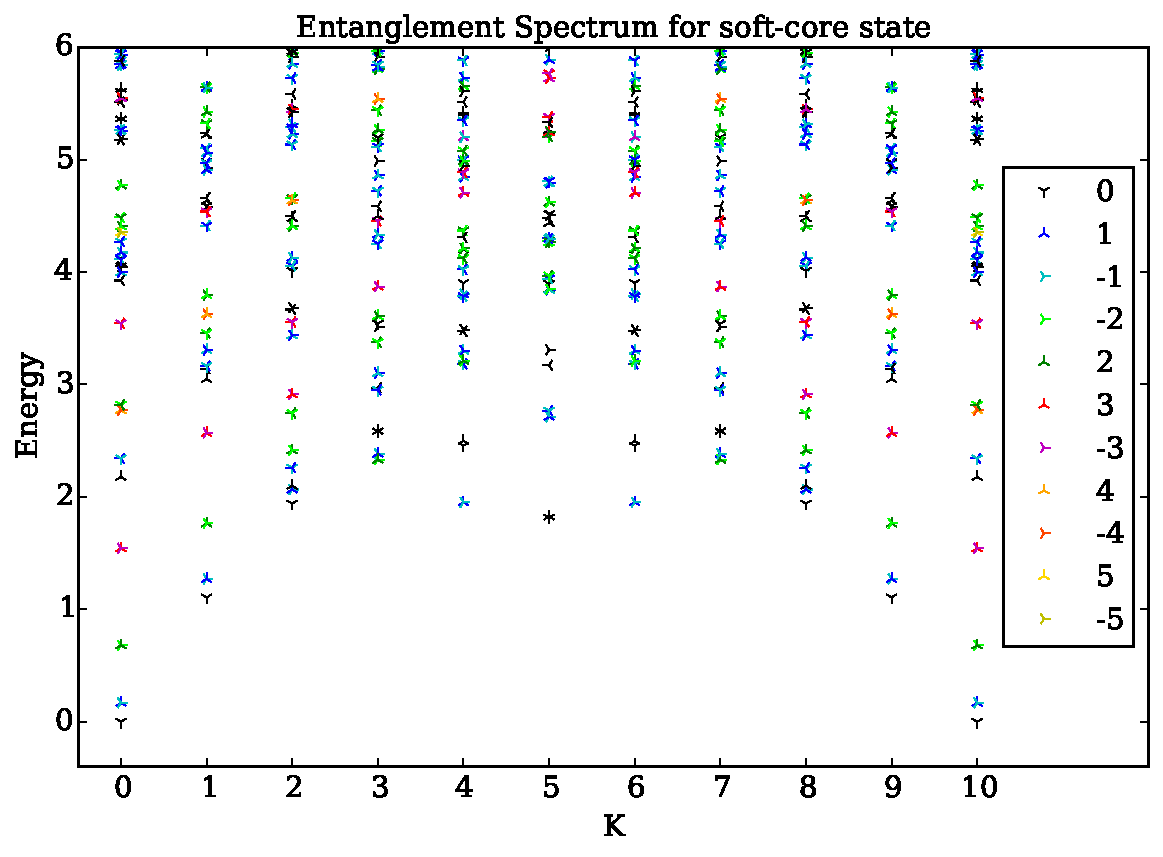
\includegraphics[width=\textwidth]{{interpolatedboson/new_plots/L_10_all_mom_10.pdf}}
\end{figure}
\end{frame}
\begin{frame}{Finite Size Analysis of Spectra}
\vskip-1.5cm
\begin{columns}[T]
    \begin{column}{.4\textwidth}
        \bi 

        \item<1-> Low energy modes show gapless $1/L$ behavior
        \item<2-> Topological entanglement entropy is 0 
        \ei
    \end{column}
    \begin{column}{.6\textwidth}
    \vskip-.3cm
        \only<1>{
        \begin{figure}[hbctp]
        \centering
        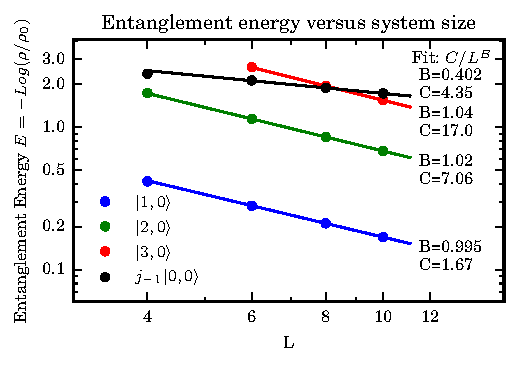
\includegraphics[width=2.5in]{{interpolatedboson/a10/plots/EntanglementEnergyScaling2.pdf}}
        %\caption{Power law fits for the lowest three states above the ground state at momentum zero and lowest two states at momentum 1 in Figure \ref{fig:sc-EEFinitesize}. The $1/L$ scaling is a signature of a gapless (entanglement) Hamiltonian. The labeling of the states $\ket{e, m}$ or $j_{-1} \ket{e, m}$ is explained in the CFT section below.}
        %\label{fig:sc-EEScaling}
        \end{figure}
        }
    \end{column}
\end{columns}
\end{frame}
\begin{frame}{Identifying CFTs: Measuring c}
\vskip-1.5cm
\begin{figure}[hbctp]
\centering
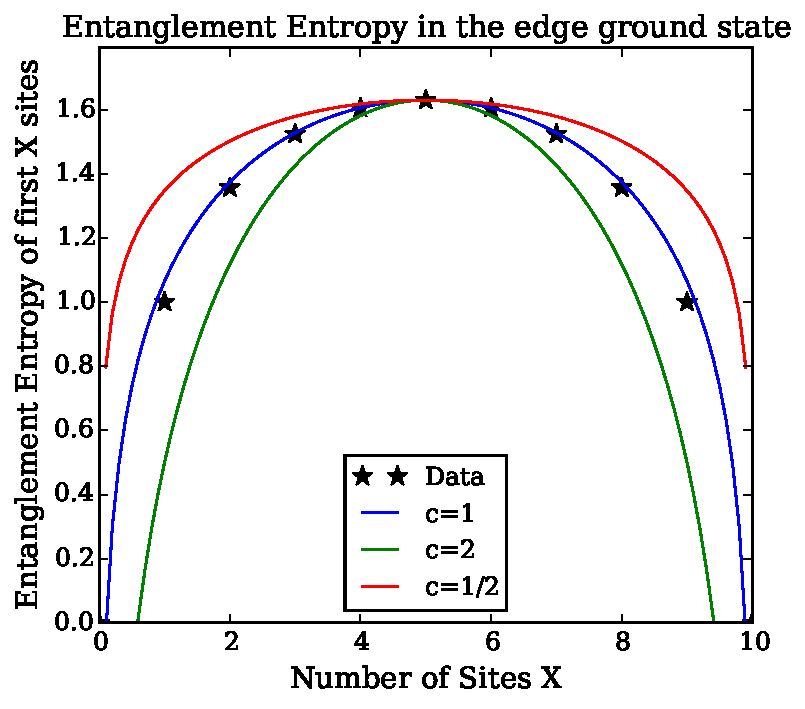
\includegraphics[height=\textheight]{{interpolatedboson/a0/plots/edge_gs_EE.pdf}}
\caption{Entanglement entropy within the entanglement ground state of the soft-core boson state on $10$ sites. For comparison, the Cardy-Calabrese formula $S(x) = c/3 \log \sin( \pi x/L) + const.$ is shown with $c=\frac{1}{2}, 1,$ and $2$, with the $const.$ fixed by matching the maximum of the entanglement entropy data. $c=1$ is a good fit.}
\label{fig:hc-edge-gs-ee}
\end{figure}
\end{frame}
\newcommand{\uL}{\mathbf{L_0}}
\newcommand{\bL}{\mathbf{\bar{L}_0}}
\begin{frame}{Level identification in CFT spectra}
\vskip-1.5cm
\only<1>{

To make a precise comparison with the free-boson CFT, we'll need to solve for (or look up) the solution of this model.

The free-boson CFT is created from the Lagrangian 
$$ \mathfrak{L} = \frac{g}{2}\int dt \int\limits_0^L dx ( \frac{1}{v^2}(\partial_t \phi)^2 - (\partial_x \phi)^2)$$
and with the compatified field identification
$$ \phi \equiv \phi + 2\pi R$$
and placed on the circle of circumference $L$ with periodic boundary conditions
$$ \phi(x) \equiv \phi(x+L).$$
}
\only<2>{
\begin{table}[h]
\centering
\begin{tabular}{c|c}
$\uL$ & $2\pi g(\frac{e}{4 \pi g R} + \frac{m R}{2})^2 + n$  \\
& \\
$\bL$ & $2\pi g(\frac{e}{4 \pi g R} - \frac{m R}{2})^2 + \bar{n}$  \\
& \\
$\mathbf{P} =\frac{2\pi v}{L}(\uL-\bL)$ & $\frac{2\pi v}{L}(em + n - \bar{n})$ \\
& \\
$\mathbf{H} = \frac{2\pi v}{L}(\uL+\bL)$ & $\frac{2\pi v}{L}(\frac{e^2}{4 \pi g R^2} + \pi g m^2 R^2 + n + \bar{n})$ \\
& \\
$\tilde{\mathbf{H}} = \frac{L}{2 \pi v \kappa}\mathbf{H}$ & $e^2 + \frac{m^2}{4 \kappa^2} + \frac{1}{\kappa}(n + \bar{n})$       
\end{tabular}
\label{Table:EV}
\caption{Eigenvalues of states $\ket{e, m}_{n, \bar{n}}$. The rescaled Hamiltonian $\tilde{\mathbf{H}}$ has eigenvalues that depend on only one free-parameter, $\kappa = 1/(4 \pi g R^2)$.(Note: A common convention is to set $g=1/4\pi$ and describe the system using $R=\sqrt{1/\kappa}$.) }
\end{table}
}

\end{frame}
\begin{frame}{Conformal Tower}
\only<1>{
\begin{figure}
    \scalebox{1}{
        \begin{tikzpicture}
\tikzstyle{yaxis} = [-triangle 90]
\tikzstyle{xaxis} = [triangle 90-triangle 90]
\node[inv](A) at (-4, 0){};
\node[inv](B) at (4, 0){};
\draw[thick, xaxis] (A)-- (B);
\node at ($ (A) !.9! (B) +(0, -1)$) {\Huge $P$};
\node[inv](A) at (0, 0){};
\node[inv](B) at (0, 4){};
\draw[thick, yaxis] (A)--(B);
\node at ($ (A) !.9! (B) +(-1, 0)$) {\Huge $E$};

\tikzset{spec/.style={circle=2pt,draw=black!100,fill=black!100,inner sep=2pt}}
\node[spec] at (0, 0){};
\node[spec] at (1, 1){};
\node[spec] at (1.8, 2){};
\node[spec] at (2.2, 2){};

\node[spec] at (2.6, 3){};
\node[spec] at (3.0, 3){};
\node[spec] at (3.4, 3){};

%\node[spec] at (-1, 1){};
%\node[spec] at (0, 2){};

%\node[] at (3, -1.5){\LARGE Band metal};
%\node[] at (3, 1.5){\LARGE Band insulator};
%\draw[] (0.5, 0) -- (5.5, 0);
\end{tikzpicture}
    }
\end{figure}
}
\only<2>{
\begin{figure}
    \scalebox{1}{
        \begin{tikzpicture}
\tikzstyle{yaxis} = [-triangle 90]
\tikzstyle{xaxis} = [triangle 90-triangle 90]
\node[inv](A) at (-4, 0){};
\node[inv](B) at (4, 0){};
\draw[thick, xaxis] (A)-- (B);
\node at ($ (A) !.9! (B) +(0, -1)$) {\Huge $P$};
\node[inv](A) at (0, 0){};
\node[inv](B) at (0, 4){};
\draw[thick, yaxis] (A)--(B);
\node at ($ (A) !.9! (B) +(-1, 0)$) {\Huge $E$};

\tikzset{spec/.style={circle=2pt,draw=black!100,fill=black!100,inner sep=2pt}}
\node[spec] at (0, 0){};
\node[spec] at (1, 1){};
\node[spec] at (1.8, 2){};
\node[spec] at (2.2, 2){};

\node[spec] at (2.6, 3){};
\node[spec] at (3.0, 3){};
\node[spec] at (3.4, 3){};

\node[spec] at (-1, 1){};
\node[spec] at (-1.8, 2){};
\node[spec] at (-2.2, 2){};

\node[spec] at (-2.6, 3){};
\node[spec] at (-3.0, 3){};
\node[spec] at (-3.4, 3){};


%\node[spec] at (-1, 1){};
%\node[spec] at (0, 2){};

%\node[] at (3, -1.5){\LARGE Band metal};
%\node[] at (3, 1.5){\LARGE Band insulator};
%\draw[] (0.5, 0) -- (5.5, 0);
\end{tikzpicture}
    }
\end{figure}
}
\only<3>{
\begin{figure}
    \scalebox{1}{
        \begin{tikzpicture}
\tikzstyle{yaxis} = [-triangle 90]
\tikzstyle{xaxis} = [triangle 90-triangle 90]
\node[inv](A) at (-4, 0){};
\node[inv](B) at (4, 0){};
\draw[thick, xaxis] (A)-- (B);
\node at ($ (A) !.9! (B) +(0, -1)$) {\Huge $P$};
\node[inv](A) at (0, 0){};
\node[inv](B) at (0, 4){};
\draw[thick, yaxis] (A)--(B);
\node at ($ (A) !.9! (B) +(-1, 0)$) {\Huge $E$};

\tikzset{spec/.style={circle=2pt,draw=black!100,fill=black!100,inner sep=2pt}}
\node[spec] at (0, 0){};
\node[spec] at (1, 1){};
\node[spec] at (1.8, 2){};
\node[spec] at (2.2, 2){};

\node[spec] at (2.6, 3){};
\node[spec] at (3.0, 3){};
\node[spec] at (3.4, 3){};

\node[spec] at (0-1, 0+1){};
\node[spec] at (1-1, 1+1){};
\node[spec] at (1.8-1, 2+1){};
\node[spec] at (2.2-1, 2+1){};

\node[spec] at (2.6-1, 3+1){};
\node[spec] at (3.0-1, 3+1){};
\node[spec] at (3.4-1, 3+1){};

% \node[spec] at (0-2, 0+2){};
% \node[spec] at (1-2, 1+2){};
% \node[spec] at (1.8-2, 2+2){};
% \node[spec] at (2.2-2, 2+2){};

\node[spec] at (-1, 1){};
\node[spec] at (-1.8, 2){};
\node[spec] at (-2.2, 2){};

\node[spec] at (-2.6, 3){};
\node[spec] at (-3.0, 3){};
\node[spec] at (-3.4, 3){};


%\node[spec] at (-1, 1){};
%\node[spec] at (0, 2){};

%\node[] at (3, -1.5){\LARGE Band metal};
%\node[] at (3, 1.5){\LARGE Band insulator};
%\draw[] (0.5, 0) -- (5.5, 0);
\end{tikzpicture}
    }
\end{figure}
}
\only<4>{
\begin{figure}
    \scalebox{1}{
        \begin{tikzpicture}
\tikzstyle{yaxis} = [-triangle 90]
\tikzstyle{xaxis} = [triangle 90-triangle 90]
\node[inv](A) at (-4, 0){};
\node[inv](B) at (4, 0){};
\draw[thick, xaxis] (A)-- (B);
\node at ($ (A) !.9! (B) +(0, -1)$) {\Huge $P$};
\node[inv](A) at (0, 0){};
\node[inv](B) at (0, 4){};
\draw[thick, yaxis] (A)--(B);
\node at ($ (A) !.9! (B) +(-1, 0)$) {\Huge $E$};

\tikzset{spec/.style={circle=2pt,draw=black!100,fill=black!100,inner sep=2pt}}
\node[spec] at (0, 0){};
\node[spec] at (1, 1){};
\node[spec] at (1.8, 2){};
\node[spec] at (2.2, 2){};

\node[spec] at (2.6, 3){};
\node[spec] at (3.0, 3){};
\node[spec] at (3.4, 3){};

\node[spec] at (0-1, 0+1){};
\node[spec] at (1-1, 1+1){};
\node[spec] at (1.8-1, 2+1){};
\node[spec] at (2.2-1, 2+1){};

\node[spec] at (2.6-1, 3+1){};
\node[spec] at (3.0-1, 3+1){};
\node[spec] at (3.4-1, 3+1){};

\node[spec] at (0-2.2, 0+2){};
\node[spec] at (1-2.2, 1+2){};
\node[spec] at (1.8-2.3, 2+2){};
\node[spec] at (2.2-2.1, 2+2){};

\node[spec] at (0-1.8, 0+2){};
\node[spec] at (1-1.8, 1+2){};
\node[spec] at (1.8-2, 2+2){};
\node[spec] at (2.2-1.8, 2+2){};

\node[spec] at (-2.6, 3){};
\node[spec] at (-3.0, 3){};
\node[spec] at (-3.4, 3){};

\node[spec] at (-2.6+1, 4){};
\node[spec] at (-3.0+1, 4){};
\node[spec] at (-3.4+1, 4){};


\end{tikzpicture}
    }
\end{figure}
}
\end{frame}
\newcommand{\uL}{\mathbf{L_0}}
\newcommand{\bL}{\mathbf{\bar{L}_0}}
\begin{frame}{Level identification in CFT spectra}
\vskip-1.5cm
\begin{table}[h]
\centering
\begin{tabular}{c|c}

$\mathbf{P} =\frac{2\pi}{L}(\uL-\bL)$ & 
$\frac{2\pi}{L}(em + n - \bar{n})$ \\
&
\\
$\widetilde{\mathbf{P}}$  &
$(em + n - \bar{n})$\\
& 
\\
$\mathbf{H} = \frac{2\pi}{L}(\uL+\bL)$ &
 $\frac{2\pi}{L}(\frac{\kappa e^2}{2} + \frac{m^2}{2 \kappa} + \frac{n + \bar{n}}{2})$ \\
&
 \\
$\widetilde{\mathbf{H}} = \frac{L}{2 \pi \kappa}\mathbf{H}$ &
 $e^2 + \frac{m^2}{4 \kappa^2} + \frac{1}{\kappa}(n + \bar{n})$       
\end{tabular}
\label{Table:EV}
\caption{Eigenvalues of states $\ket{e, m}_{n, \bar{n}}$.} 
\end{table}

The rescaled Hamiltonian $\widetilde{\mathbf{H}}$ has eigenvalues that depend on only one free-parameter, $\kappa = 1/(4 \pi g R^2)$.

\end{frame}

\begin{frame}{Level identification in CFT spectra}
\vskip-1.5cm
\begin{columns}[T]
\begin{column}{0.25\textwidth}
\begin{figure}
\scalebox{0.5}{
\begin{tikzpicture}[x=30mm,y=25mm]
\tikzstyle{yaxis} = [-triangle 90]
\tikzstyle{xaxis} = [triangle 90-triangle 90]
\node[inv](A) at (-.5, 0){};
\node[inv](B) at (2.5, 0){};
\draw[thick, xaxis] (A)-- (B);
\node at ($ (A) !.6! (B) +(0, -0.3)$) {\Huge $P$ \Large (in units of $\frac{2\pi}{L}$)};
\node[inv](A) at (0, 0){};
\node[inv](B) at (0, 4){};
\draw[thick, yaxis] (A)--(B);
\node at ($ (A) !.9! (B) +(-0.3, 0)$) {\Huge $E$};

\def\rs{{ 0, 1, 0, .9, 0, 1, 1}}
\def\gs{{0, 0, 0, .5, 1, 1, 0}}
\def\bs{{0, 0, 1, 0, 0, 0, 1}}
\def\decxs{{1,1.95,2.05,0}}
\def\decys{{1, 2,    2, 2}}

\foreach \q in {6, ..., 0}{
\pgfmathparse{\rs[\q]}
\edef\r{\pgfmathresult}

\pgfmathparse{\gs[\q]}
\edef\g{\pgfmathresult}

\pgfmathparse{\bs[\q]}
\edef\b{\pgfmathresult}
\definecolor{mycolor}{rgb}{\r,\g,\b}
\tikzset{spec/.style={circle=2pt,draw=black!100,fill=mycolor!100,inner sep=2pt}}
\node[spec](P\q) at (0, 1/6.2*\q*\q*1/4.0){};
\foreach \k in {0,...,3}{

\pgfmathparse{\decxs[\k]}
\edef\x{\pgfmathresult}
\pgfmathparse{\decys[\k]}
\edef\y{\pgfmathresult}

%\pgfmathtruncatemacro\intx{\x}
%\pgfmathtruncatemacro\inty{\y}

\node[spec](P\q\k) at ($(P\q)+(\x, \y)$){};
%\node[spec](P\q\k) at ($(P\q)+(-\x, \y)$){};
% \newdimen\xx
% \newdimen\yy
% \pgfextractx{\xx}{\pgfpointanchor{P\q\k}{center}}
% \pgfextracty{\yy}{\pgfpointanchor{P\q\k}{center}}
% \pgfmathtruncatemacro\intx{\xx}
% \pgfmathtruncatemacro\inty{\yy}


}
}

\end{tikzpicture}
}
\end{figure}
\end{column}
\begin{column}{0.75\textwidth}
\begin{figure}[hbctp]
\begin{center}
\includegraphics[height=\textheight]{{interpolatedboson/a10/plots/EEIdentify.pdf}}
\end{center}
%\caption{The identification of the states $\ket{e, m}_{n, \bar{n}}$ in the spectrum of the soft-core boson entanglement Hamiltonian. The label $e$ gives the U(1) charge. The labels $n$, $\bar{n}$ label the levels in the right or left-moving sectors of the Kac-Moody algebra. When the level $n$ is larger than 1, the level shows $Z(n)$ approximately degenerate states. The best estimate for the Luttinger parameter $\kappa = 1/6.4$ is given by the inverse of the energy of the $\ket{1, 0}_{1, 0}$ state. The label $m$ is 0 for all states shown - however, the primary states $\ket{e, m=\pm 1}$ can be seen centered around momentum $\pi$, with energies on the order of $1/(4\kappa^2)$.}
%\label{fig:primaries}
\end{figure}
\end{column}
\end{columns}
\end{frame}
%%\newcommand{\uL}{\mathbf{L_0}}
%\newcommand{\bL}{\mathbf{\bar{L}_0}}
\begin{frame}{Level identification in CFT spectra}
\vskip-1.5cm
\begin{figure}[hbctp]
\begin{center}
\includegraphics[height=\textheight]{{interpolatedboson/a10/plots/EEIdentify.pdf}}
\end{center}
%\caption{The identification of the states $\ket{e, m}_{n, \bar{n}}$ in the spectrum of the soft-core boson entanglement Hamiltonian. The label $e$ gives the U(1) charge. The labels $n$, $\bar{n}$ label the levels in the right or left-moving sectors of the Kac-Moody algebra. When the level $n$ is larger than 1, the level shows $Z(n)$ approximately degenerate states. The best estimate for the Luttinger parameter $\kappa = 1/6.4$ is given by the inverse of the energy of the $\ket{1, 0}_{1, 0}$ state. The label $m$ is 0 for all states shown - however, the primary states $\ket{e, m=\pm 1}$ can be seen centered around momentum $\pi$, with energies on the order of $1/(4\kappa^2)$.}
%\label{fig:primaries}
\end{figure}
\end{frame}
\begin{frame}{Goals for Honeycomb Mott Insulator}
\vskip-1.5cm
\begin{block}{Completed}
\bi 
\item Build a tensor network representation for doing computations
\item  Verify that no spontaneous symmetry breaking occurs
%We'll do this by computing correlation functions on a cylinder geometry combined with scaling analysis in the circumference

\item Rule out topological order

\item Compute entanglement spectrum to check for nontrivial entanglement

\ei 
\end{block}
\begin{block}{Not Yet}
\bi
\item Understand the role of symmetries in protecting entanglement in interacting quasi-1D and 2D theories
\item Find distinguishing topological invariant and/or physical signatures
\item Find a parent Hamiltonian 
\ei
\end{block}
\end{frame}
\begin{frame}{Open questions and speculation}
Correspondence between edge and bulk physics
In a RG-fixed point tensor network state (such as toric code):
Can 
\end{frame}
\section*{}

\frame{
  \vspace{2cm}
  {\huge Questions?}

  \vspace{3cm}
  \begin{flushright}
    Brayden Ware

    \structure{\footnotesize{brayden@physics.ucsb.edu}}
  \end{flushright}
}

\frame{
  \vfill
  \centering
  \highlighton{
  \usebeamerfont*{frametitle}Bonus slides

  %\usebeamerfont*{framesubtitle}Bonus slides
  }
  \vfill
}

\begin{frame}
  \frametitle{Resources}
  \vskip-1.7cm
  %\framesubtitle{If you want to improve this style}
  \bibliography{references}
  %\beamertemplatearticlebibitems
\end{frame}


\begin{frame}{Bulk Entanglement and Edges}
%We can (heuristically for now) connect the existence of the edge state to the idea that these types of insulators are really distinct from atomic insulators. 
\vskip-1.5cm
Bulk ground state contains information about edge physics
\bi
\item  Imagine cutting IQH state in half, forming edge states $\ket{k}_{L, R}$
%or another state with a protected edge
%at this point, the eigenstates of the system are factored between left and right sides
% the lowest energy states look like ground states far away, but differ at the edge due to the edge modes 
\item Adiabatically tune the coupling back to normal value 
%and find the new ground state
\item System can lower its energy by coupling the currents
\item Entangled eigenstate $\sum \ket{k}_L \otimes\ket{-k}_R$ 
% But this is just the regular state of the system with no cut at all!
\item Atomic insulator wavefunctions factor trivially - no entanglement.
% This suggests that these are distinct phases of matter from atomic insulators, we should look at entanglement and show that the entanglement is robust to perturbations. This can be a route to showing the edge is robust to (certain) perturbations without having to worry about the actual precise form of the edge.  
\ei 
\vskip-0.2cm
\begin{figure}
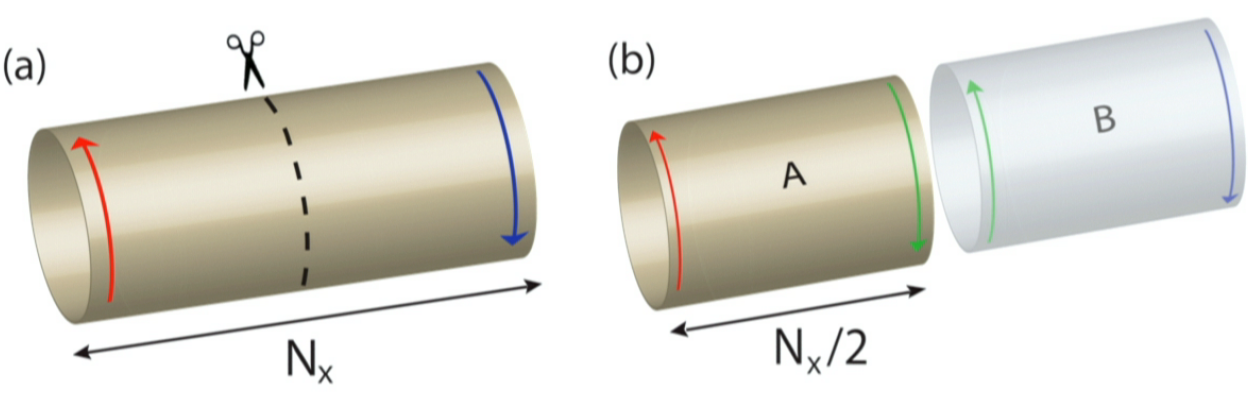
\includegraphics[width=\linewidth]{diagrams/entanglement_cut.png}
\end{figure}
\footnotetext[3]{
\citep{Alexandradinata2011-os}} 
\end{frame}


\begin{frame}{MPS Example: AKLT State}
\vskip-1.5cm
\begin{block}{Haldane Phase for Spin-1 chains $(j=1, m=0)$}
\vskip-0.8cm
$$
H_{AKLT} = \sum\limits_{i} J \vec{S}_i\cdot \vec{S}_{i+1} + J' (\vec{S}_i\cdot \vec{S}_{i+1})^2 + D (S^z_i)^2+BS^x
$$
\end{block}
\begin{columns}[T]
    \begin{column}[T]{.45\textwidth}
        \vskip-1.2cm
        \begin{figure}
        \centering
        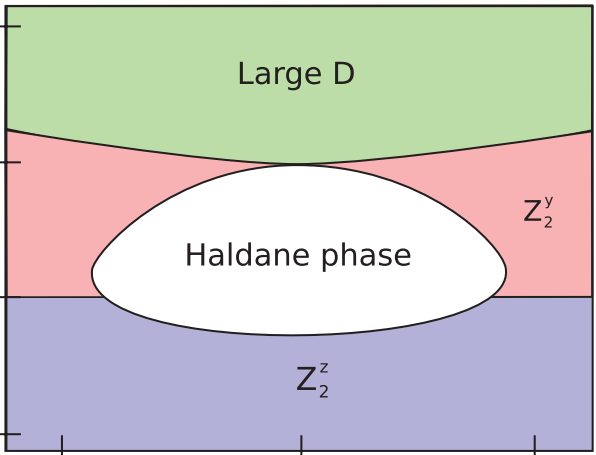
\includegraphics[width=\columnwidth]{diagrams/aklt2.png}
        \end{figure}
    \end{column}
    \begin{column}[T]{.55\textwidth}
    \vskip-0.8cm
    Two distinct featureless insulators:
    \bi 
    \item Large-D phase
    \bi 
    \item Contains product state wavefunction $\ket{\psi} = \ket{000...}$ 
    \ei
    \item Haldane phase
    \bi 
    \item Contains AKLT wavefunction $\ket{\psi} = \Sigma\ket{+00-0+...}$
    \ei 
        \begin{figure}[h]
            \hspace{-2cm}
            \scalebox{1.2}{
            \begin{frame}{MPS Example: AKLT State}
\vskip-1.5cm
\begin{block}{Haldane Phase for Spin-1 chains $(j=1, m=0)$}
\vskip-0.8cm
$$
H_{AKLT} = \sum\limits_{i} J \vec{S}_i\cdot \vec{S}_{i+1} + J' (\vec{S}_i\cdot \vec{S}_{i+1})^2 + D (S^z_i)^2+BS^x
$$
\end{block}
\begin{columns}[T]
    \begin{column}[T]{.45\textwidth}
        \vskip-1.2cm
        \begin{figure}
        \centering
        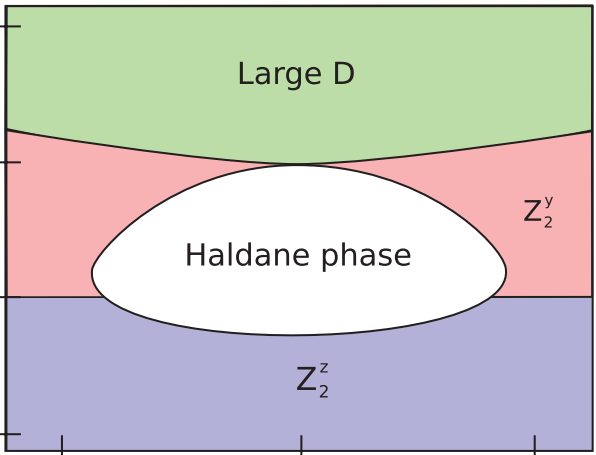
\includegraphics[width=\columnwidth]{diagrams/aklt2.png}
        \end{figure}
    \end{column}
    \begin{column}[T]{.55\textwidth}
    \vskip-0.8cm
    Two distinct featureless insulators:
    \bi 
    \item Large-D phase
    \bi 
    \item Contains product state wavefunction $\ket{\psi} = \ket{000...}$ 
    \ei
    \item Haldane phase
    \bi 
    \item Contains AKLT wavefunction $\ket{\psi} = \Sigma\ket{+00-0+...}$
    \ei 
        \begin{figure}[h]
            \hspace{-2cm}
            \scalebox{1.2}{
            \begin{frame}{MPS Example: AKLT State}
\vskip-1.5cm
\begin{block}{Haldane Phase for Spin-1 chains $(j=1, m=0)$}
\vskip-0.8cm
$$
H_{AKLT} = \sum\limits_{i} J \vec{S}_i\cdot \vec{S}_{i+1} + J' (\vec{S}_i\cdot \vec{S}_{i+1})^2 + D (S^z_i)^2+BS^x
$$
\end{block}
\begin{columns}[T]
    \begin{column}[T]{.45\textwidth}
        \vskip-1.2cm
        \begin{figure}
        \centering
        \includegraphics[width=\columnwidth]{diagrams/aklt2.png}
        \end{figure}
    \end{column}
    \begin{column}[T]{.55\textwidth}
    \vskip-0.8cm
    Two distinct featureless insulators:
    \bi 
    \item Large-D phase
    \bi 
    \item Contains product state wavefunction $\ket{\psi} = \ket{000...}$ 
    \ei
    \item Haldane phase
    \bi 
    \item Contains AKLT wavefunction $\ket{\psi} = \Sigma\ket{+00-0+...}$
    \ei 
        \begin{figure}[h]
            \hspace{-2cm}
            \scalebox{1.2}{
            \input{diagrams/aklt.tex}
            }
        \end{figure}

    \ei
    \end{column}
\end{columns}

\end{frame}
            }
        \end{figure}

    \ei
    \end{column}
\end{columns}

\end{frame}
            }
        \end{figure}

    \ei
    \end{column}
\end{columns}

\end{frame}
\begin{frame}{1D SPT Example: AKLT State}
\vskip-1.5cm
\only<1>{
\begin{figure}
\scalebox{2}{
            \begin{frame}{MPS Example: AKLT State}
\vskip-1.5cm
\begin{block}{Haldane Phase for Spin-1 chains $(j=1, m=0)$}
\vskip-0.8cm
$$
H_{AKLT} = \sum\limits_{i} J \vec{S}_i\cdot \vec{S}_{i+1} + J' (\vec{S}_i\cdot \vec{S}_{i+1})^2 + D (S^z_i)^2+BS^x
$$
\end{block}
\begin{columns}[T]
    \begin{column}[T]{.45\textwidth}
        \vskip-1.2cm
        \begin{figure}
        \centering
        \includegraphics[width=\columnwidth]{diagrams/aklt2.png}
        \end{figure}
    \end{column}
    \begin{column}[T]{.55\textwidth}
    \vskip-0.8cm
    Two distinct featureless insulators:
    \bi 
    \item Large-D phase
    \bi 
    \item Contains product state wavefunction $\ket{\psi} = \ket{000...}$ 
    \ei
    \item Haldane phase
    \bi 
    \item Contains AKLT wavefunction $\ket{\psi} = \Sigma\ket{+00-0+...}$
    \ei 
        \begin{figure}[h]
            \hspace{-2cm}
            \scalebox{1.2}{
            \begin{frame}{MPS Example: AKLT State}
\vskip-1.5cm
\begin{block}{Haldane Phase for Spin-1 chains $(j=1, m=0)$}
\vskip-0.8cm
$$
H_{AKLT} = \sum\limits_{i} J \vec{S}_i\cdot \vec{S}_{i+1} + J' (\vec{S}_i\cdot \vec{S}_{i+1})^2 + D (S^z_i)^2+BS^x
$$
\end{block}
\begin{columns}[T]
    \begin{column}[T]{.45\textwidth}
        \vskip-1.2cm
        \begin{figure}
        \centering
        \includegraphics[width=\columnwidth]{diagrams/aklt2.png}
        \end{figure}
    \end{column}
    \begin{column}[T]{.55\textwidth}
    \vskip-0.8cm
    Two distinct featureless insulators:
    \bi 
    \item Large-D phase
    \bi 
    \item Contains product state wavefunction $\ket{\psi} = \ket{000...}$ 
    \ei
    \item Haldane phase
    \bi 
    \item Contains AKLT wavefunction $\ket{\psi} = \Sigma\ket{+00-0+...}$
    \ei 
        \begin{figure}[h]
            \hspace{-2cm}
            \scalebox{1.2}{
            \input{diagrams/aklt.tex}
            }
        \end{figure}

    \ei
    \end{column}
\end{columns}

\end{frame}
            }
        \end{figure}

    \ei
    \end{column}
\end{columns}

\end{frame}
            }
\end{figure}
\begin{columns}[T]
\begin{column}[T]{.5\textwidth}
\vskip-1.5cm
\begin{figure}
\includegraphics[width=\columnwidth]{diagrams/aklt2.png}
\end{figure}
\end{column}
   \begin{column}[T]{.5\textwidth}
   \vskip-1cm
    \includegraphics[width=\columnwidth]{diagrams/akltEE.png}
    \end{column}
\end{columns}
}
Haldane phase distinguished by exact double degeneracy in entire  entanglement spectrum.

\only<2>{
\begin{figure}
\includegraphics[width=\textwidth]{diagrams/akltchart.png}
\end{figure}
}
\end{frame}
\begin{frame}{Technical Slide: Threading Flux in a MPS}

\begin{figure}[h]
    \centering
    \scalebox{1}{
    \begin{tikzpicture}[node distance=0.4cm]
\begin{scope}[decoration={
    markings,
    mark=at position 0.5 with {\arrow{>}}}
    ]
\foreach \i in {1,...,5} {
	\node[gamma] (G\i) at (1.5*\i,0) {};
	\node (l\i) at ($ (G\i) + (0, 1) $) {$p_\i$};
	\draw[thick] (G\i) -- (l\i);
	\node[below of=G\i] {$A^\i$};
}
\foreach \i / \j in {1/2,2/3,3/4,4/5} {
	\draw[thick, postaction={decorate}] (G\j) -- (G\i);
}
\node[side] (B) at (0.5, 0) {$B$};
%\node (b1) at (0, 0) {$b_1$};
\draw[thick, postaction={decorate}] (G1) -- node[below]{$b_0$}(B);
\draw[thick, postaction={decorate}] (8.1, 0)--(G5.east);
\draw[thick, postaction={decorate}] (B.west) -- node[below]{$b_1$}(-0.1, 0);
\end{scope}
\draw[thick, dashed] (0.2,0) .. controls (-1,0) and (-0.6,0.6) .. (4,0.5) .. controls (8.5,0.5) and (9,0) .. (7.5,0);
\end{tikzpicture}
    }
\end{figure}

$$
\ket{\psi} = \sum\limits_{p_1 ... p_5}   Tr(B A^{p_1}_1 ... A^{p_5}_5)\ket{p_1 ... p_5} 
$$

Flux threading = twist in boundary conditions
Applications of flux threading: 
Proof of LSM Theorem  and extensions
Detecting 2D SPT order on a cylinder

\end{frame}
\begin{frame}{Flux-Threading Arguments for SPTs?}
\vskip-1.5cm
Recall that the boundary conditions in a MPS are set by a matrix at the edge.

\begin{figure}[h]
    \centering
    \scalebox{1}{
    \begin{tikzpicture}[node distance=0.4cm]
\begin{scope}[decoration={
    markings,
    mark=at position 0.5 with {\arrow{>}}}
    ]
\foreach \i in {1,...,5} {
	\node[gamma] (G\i) at (1.5*\i,0) {};
	\node (l\i) at ($ (G\i) + (0, 1) $) {$p_\i$};
	\draw[thick] (G\i) -- (l\i);
	\node[below of=G\i] {$A^\i$};
}
\foreach \i / \j in {1/2,2/3,3/4,4/5} {
	\draw[thick, postaction={decorate}] (G\j) -- (G\i);
}
\node[side] (B) at (0.5, 0) {$B$};
%\node (b1) at (0, 0) {$b_1$};
\draw[thick, postaction={decorate}] (G1) -- node[below]{$b_0$}(B);
\draw[thick, postaction={decorate}] (8.1, 0)--(G5.east);
\draw[thick, postaction={decorate}] (B.west) -- node[below]{$b_1$}(-0.1, 0);
\end{scope}
\draw[thick, dashed] (0.2,0) .. controls (-1,0) and (-0.6,0.6) .. (4,0.5) .. controls (8.5,0.5) and (9,0) .. (7.5,0);
\end{tikzpicture}
    }
\end{figure}

Inserting the group operation $V_g$ on a single link in a periodic chain is the same as changing the boundary conditions. This is an operational procedure for 'threading a flux' that works in interacting theories or even with then symmetry is inversion or time-reversal.

The edge action can be interpreted as a 'composition of fluxes' $V_g V_h = \exp{i \omega(g, h)} V_{gh}$.
\end{frame}
\begin{frame}{Symmetry Protected Entanglement in 1D}
\vskip-1.5cm

\begin{alert}{Touch on inversion symmetry?}
\end{alert}

\bi 
\item These edge symmetries $V_g$ commute with the 'reduced density matrix' $\tilde{\rho}_L$ of the system and thus only act non-trivially on degenerate entanglement spectra eigenvalues. 

\item Because the classes of projective symmetry groups are discrete, you can't change the action on the edge continuously between classes (without going through a phase transition.)
\ei 

\end{frame}
\begin{frame}{Properties of Featureless MPS}
\vskip-1.5cm
MPS for featureless 1D or quasi-1D systems have non-degenerate transfer matrices and are called simple. Simple MPS can be proved to have:

\bi 
\item Correlations are insensitive to boundary conditions
\item Can construct a featureless 'parent Hamiltonian' 
\note{from the wavefunction alone}
\item Two simple MPS with equal wavefunctions are (uniquely) gauge equivalent
\item Corollary: Edges can be labeled with a (possibly projective) representation of the group of physical symmetries.

\begin{figure}
\scalebox{1}{
            \begin{tikzpicture}
\tikzset{gamma/.style={circle=2pt,draw=black!100, very thick, fill=blue!40, inner sep=2pt}}
\tikzset{box/.style={draw, inner sep = 2pt}}
\begin{scope}[very thick,decoration={
    markings,
    mark=at position 0.5 with {\arrow{<}}}
    ] 
    
\pgfmathsetmacro{\left}{-1.3}
\pgfmathsetmacro{\center}{0}
\pgfmathsetmacro{\right}{2}

\pgfmathsetmacro{\bond}{0.3}

\node[box] (Ug) at (\left, 0.8) {$U_g$};
\node[gamma] (A1) at (\left, 0) {$\Gamma$};

\draw[thick, postaction={decorate}] ($(A1.west) + (-\bond, 0) $) -- (A1.west);
\draw[thick, postaction={decorate}] (A1.east) -- node[right] {} +(\bond,0);


\node at (\center, 0.1){\large $ = e^{i \theta_g}$};    


\node[gamma] (A) at (\right, 0) {$\Gamma$};
\node[box] (VL) at ($(A) + (-0.8, 0) $) {$V_{gI}$};
\node[box] (VR) at ($(A) + (0.8, 0) $) {$V_{gI}^{\dagger}$};
\draw[thick, postaction={decorate}]  ($(VL.west)+(-\bond, 0)$) -- (VL.west);
\draw[thick, postaction={decorate}] (VR.east) -- ($(VR.east)+(\bond, 0)$);
\draw[thick, postaction={decorate}] (VL) -- (A);
\draw[thick, postaction={decorate}] (A) -- (VR);

\end{scope}
\begin{scope}[very thick,decoration={
    markings,
    mark=at position 0.5 with {\arrow{>}}}
    ] 
\pgfmathsetmacro{\bond}{0.3}
\draw[thick, postaction={decorate}] (A1)--(Ug);
\draw[thick, postaction={decorate}] (Ug.north) -- node[above] {} +(0,\bond);
\draw[thick, postaction={decorate}] (A.north) -- node[above] {} +(0,\bond);
\end{scope}
\end{tikzpicture}
            }
\end{figure}

\item Bonus: we can determine $V_g$ by diagonalizing the transfer matrix with the insertion $U_g$. 

\ei 

\note{
Transfer matrix becomes degenerate when 
\bi 
\item 
\item Correlations in spontaneous symmetry breaking MPS have extreme senstivity to boundary conditions
\item Correlations in topological ordered state (on large enough cylinder) completely insensitive to boundary conditions when operators don't wrap around cylinder.
\item Gapless 2D PEPS on cylinder?

\item Notes on phase transitions in MPS?
\ei 
}
\end{frame}
\end{document}
